% Options for packages loaded elsewhere
\PassOptionsToPackage{unicode}{hyperref}
\PassOptionsToPackage{hyphens}{url}
%
\documentclass[
]{article}
\title{nuclear energy in comparison}
\author{}
\date{\vspace{-2.5em}}

\usepackage{amsmath,amssymb}
\usepackage{lmodern}
\usepackage{iftex}
\ifPDFTeX
  \usepackage[T1]{fontenc}
  \usepackage[utf8]{inputenc}
  \usepackage{textcomp} % provide euro and other symbols
\else % if luatex or xetex
  \usepackage{unicode-math}
  \defaultfontfeatures{Scale=MatchLowercase}
  \defaultfontfeatures[\rmfamily]{Ligatures=TeX,Scale=1}
\fi
% Use upquote if available, for straight quotes in verbatim environments
\IfFileExists{upquote.sty}{\usepackage{upquote}}{}
\IfFileExists{microtype.sty}{% use microtype if available
  \usepackage[]{microtype}
  \UseMicrotypeSet[protrusion]{basicmath} % disable protrusion for tt fonts
}{}
\makeatletter
\@ifundefined{KOMAClassName}{% if non-KOMA class
  \IfFileExists{parskip.sty}{%
    \usepackage{parskip}
  }{% else
    \setlength{\parindent}{0pt}
    \setlength{\parskip}{6pt plus 2pt minus 1pt}}
}{% if KOMA class
  \KOMAoptions{parskip=half}}
\makeatother
\usepackage{xcolor}
\IfFileExists{xurl.sty}{\usepackage{xurl}}{} % add URL line breaks if available
\IfFileExists{bookmark.sty}{\usepackage{bookmark}}{\usepackage{hyperref}}
\hypersetup{
  pdftitle={nuclear energy in comparison},
  hidelinks,
  pdfcreator={LaTeX via pandoc}}
\urlstyle{same} % disable monospaced font for URLs
\usepackage[left=0.5cm,right=0.5cm,top=0.5cm,bottom=0.5cm]{geometry}
\usepackage{graphicx}
\makeatletter
\def\maxwidth{\ifdim\Gin@nat@width>\linewidth\linewidth\else\Gin@nat@width\fi}
\def\maxheight{\ifdim\Gin@nat@height>\textheight\textheight\else\Gin@nat@height\fi}
\makeatother
% Scale images if necessary, so that they will not overflow the page
% margins by default, and it is still possible to overwrite the defaults
% using explicit options in \includegraphics[width, height, ...]{}
\setkeys{Gin}{width=\maxwidth,height=\maxheight,keepaspectratio}
% Set default figure placement to htbp
\makeatletter
\def\fps@figure{htbp}
\makeatother
\setlength{\emergencystretch}{3em} % prevent overfull lines
\providecommand{\tightlist}{%
  \setlength{\itemsep}{0pt}\setlength{\parskip}{0pt}}
\setcounter{secnumdepth}{-\maxdimen} % remove section numbering
\usepackage{dcolumn}
\usepackage{array}
\usepackage{pdflscape}
\newcommand{\blandscape}{\begin{landscape}}
\newcommand{\elandscape}{\end{landscape}}
\usepackage{booktabs}
\usepackage{longtable}
\usepackage{array}
\usepackage{multirow}
\usepackage{wrapfig}
\usepackage{float}
\usepackage{colortbl}
\usepackage{pdflscape}
\usepackage{tabu}
\usepackage{threeparttable}
\usepackage{threeparttablex}
\usepackage[normalem]{ulem}
\usepackage{makecell}
\usepackage{xcolor}
\ifLuaTeX
  \usepackage{selnolig}  % disable illegal ligatures
\fi

\begin{document}
\maketitle

{
\setcounter{tocdepth}{2}
\tableofcontents
}
\hypertarget{abstract}{%
\section{Abstract}\label{abstract}}

\newpage

\hypertarget{h1-nuclear-energy-will-be-seen-as-riskier-than-other-energy-technologies-in-india.-this-paper-explores-nuclear-energy-in-comparison-with-other-technologies}{%
\section{H1: Nuclear Energy will be seen as riskier than other energy
technologies in India. this paper explores nuclear energy in comparison
with other
technologies}\label{h1-nuclear-energy-will-be-seen-as-riskier-than-other-energy-technologies-in-india.-this-paper-explores-nuclear-energy-in-comparison-with-other-technologies}}

\hypertarget{likert-responses-n-2160}{%
\subsection{Likert Responses (n= 2160)}\label{likert-responses-n-2160}}

The percentages are rounded off to whole numbers.

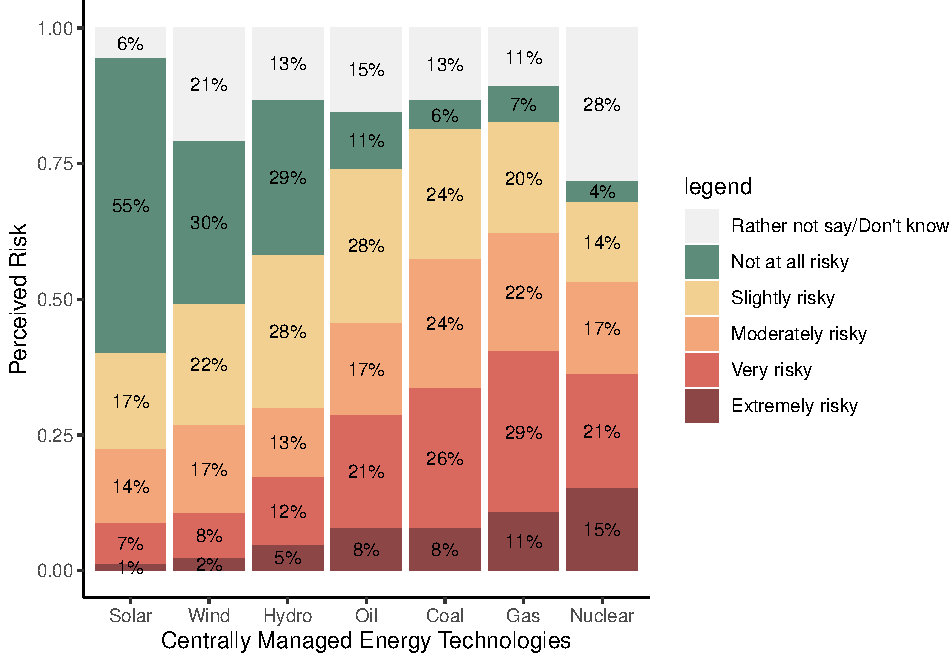
\includegraphics{nuclear-in-comparison_files/figure-latex/unnamed-chunk-5-1.pdf}
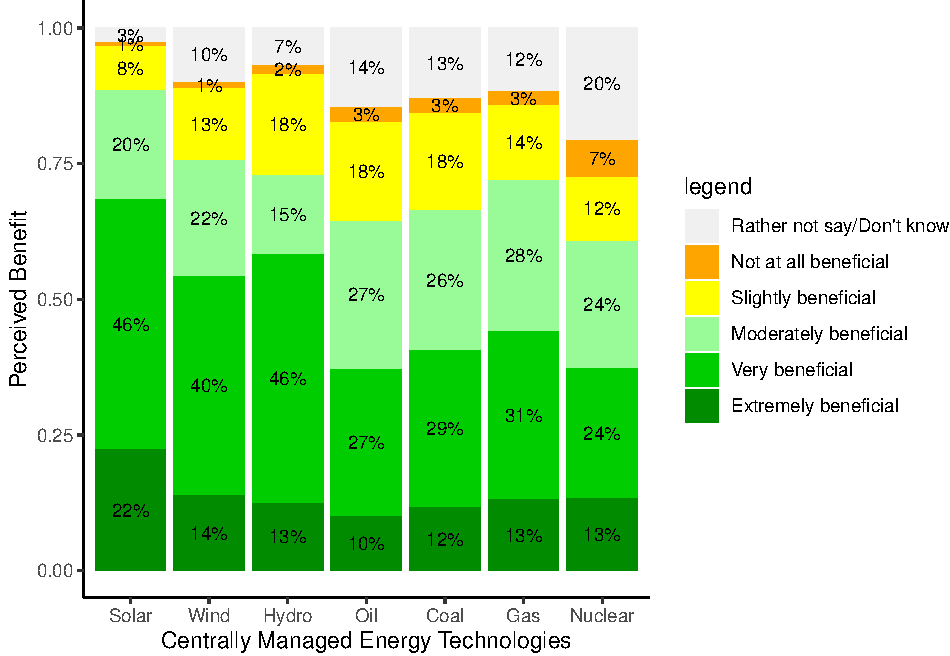
\includegraphics{nuclear-in-comparison_files/figure-latex/unnamed-chunk-5-2.pdf}

\newpage

\hypertarget{introduction-mean-perceived-risk-and-mean-perceived-benefit-for-all-energy-technologies.}{%
\subsection{Introduction: Mean Perceived Risk and Mean Perceived Benefit
for all energy
technologies.}\label{introduction-mean-perceived-risk-and-mean-perceived-benefit-for-all-energy-technologies.}}

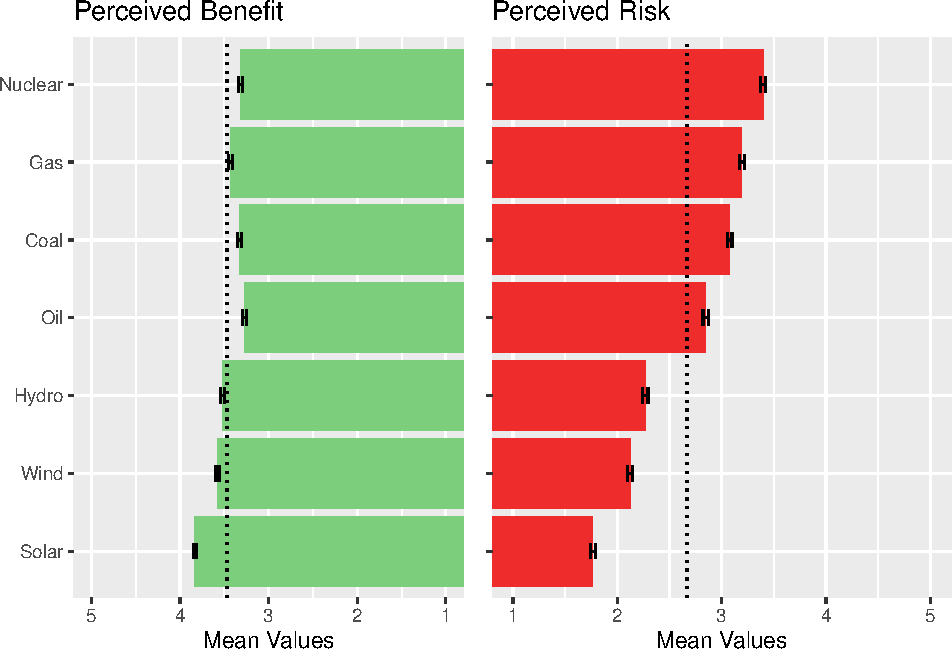
\includegraphics{nuclear-in-comparison_files/figure-latex/unnamed-chunk-7-1.pdf}

\hypertarget{boxplot-for-perceived-benefit-and-perceived-risk-by-technology}{%
\subsection{Boxplot for perceived benefit and perceived risk by
technology}\label{boxplot-for-perceived-benefit-and-perceived-risk-by-technology}}

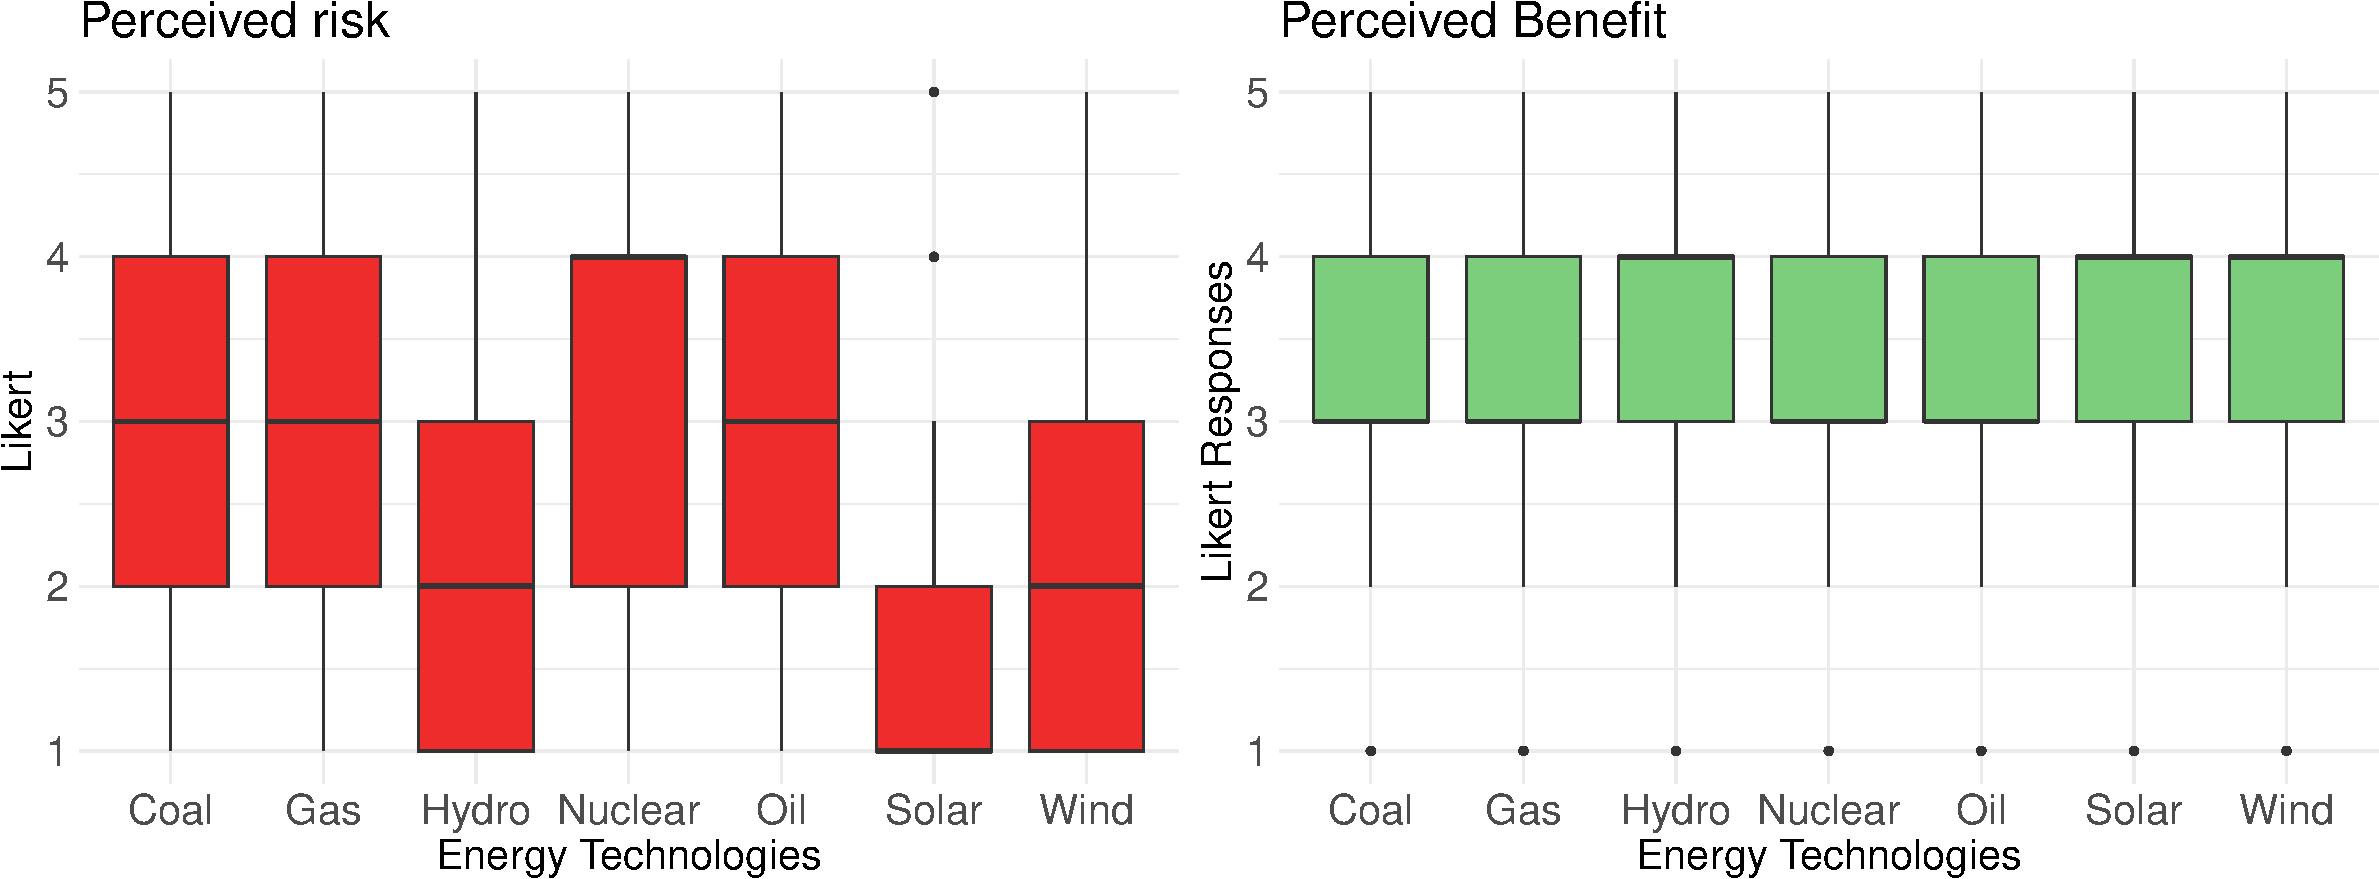
\includegraphics{nuclear-in-comparison_files/figure-latex/unnamed-chunk-8-1.pdf}

\newpage

\hypertarget{pairwise-t-test-mean-perceived-risk-and-mean-perceived-benefit-all-energy-technologies}{%
\subsection{Pairwise T-test: Mean perceived risk and mean perceived
benefit (all energy
technologies)}\label{pairwise-t-test-mean-perceived-risk-and-mean-perceived-benefit-all-energy-technologies}}

The red and green pairs indicate that there is a statistically
significant difference between the means of the two groups. White and
grey indicate - no differences between the means of the two groups.

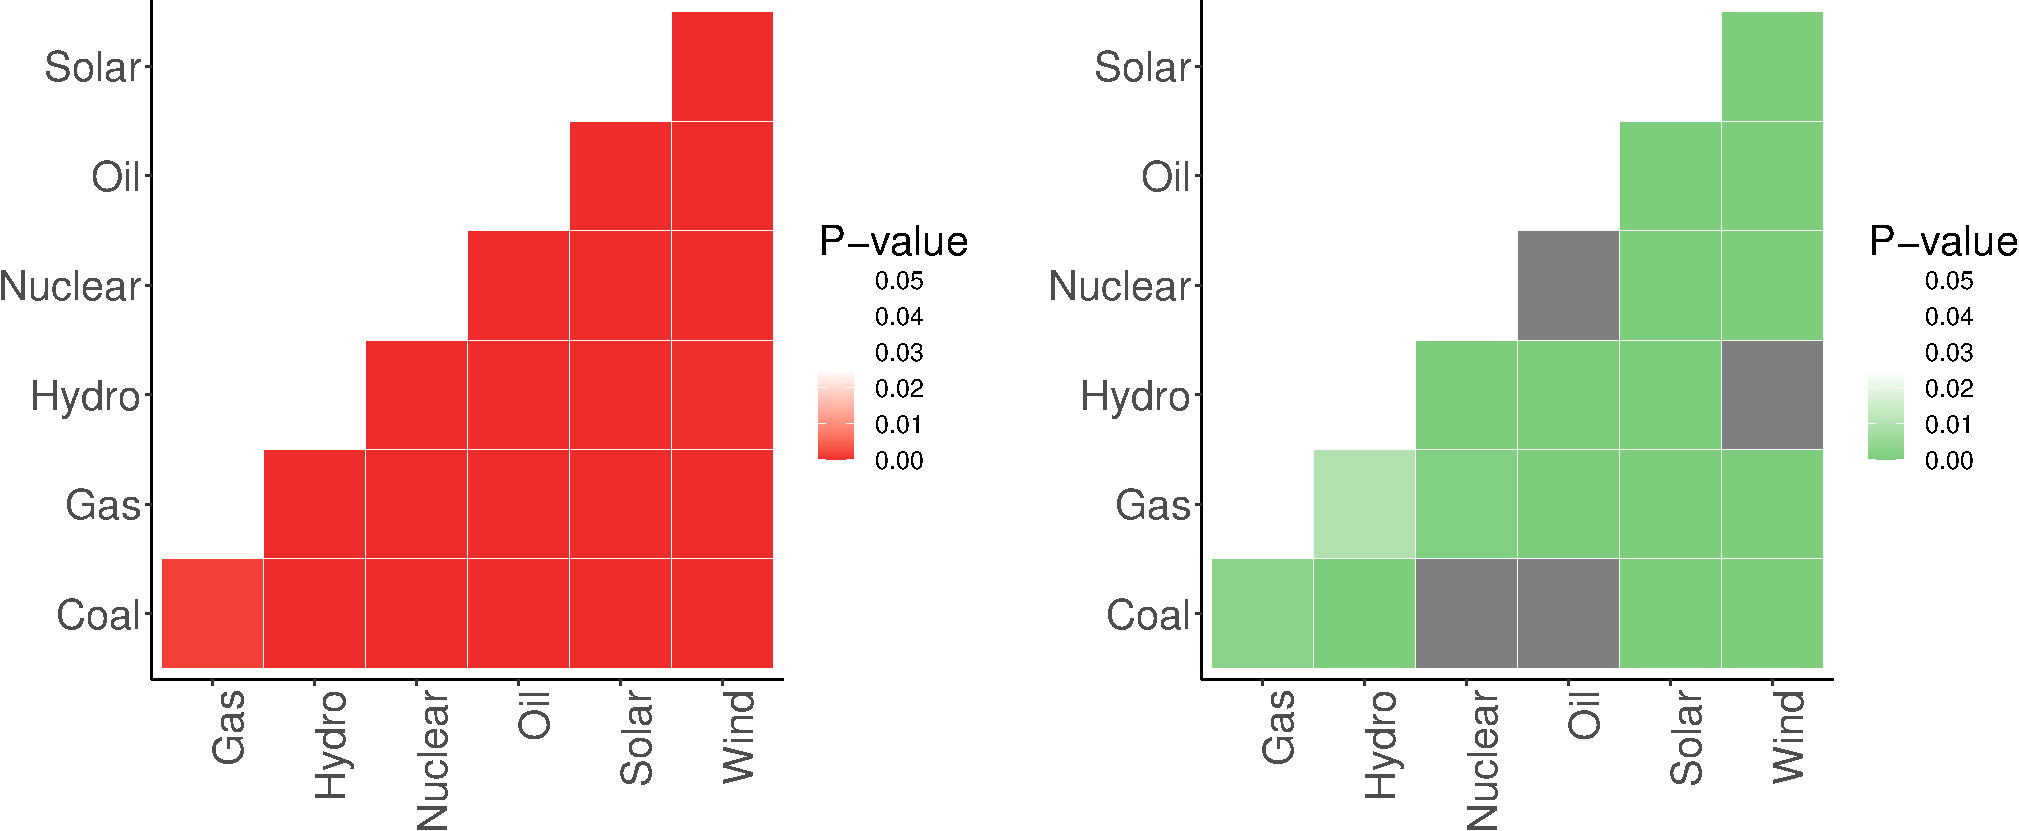
\includegraphics{nuclear-in-comparison_files/figure-latex/unnamed-chunk-9-1.pdf}

\newpage

\hypertarget{benefit---risk-for-each-technology}{%
\subsection{Benefit - Risk for each
technology}\label{benefit---risk-for-each-technology}}

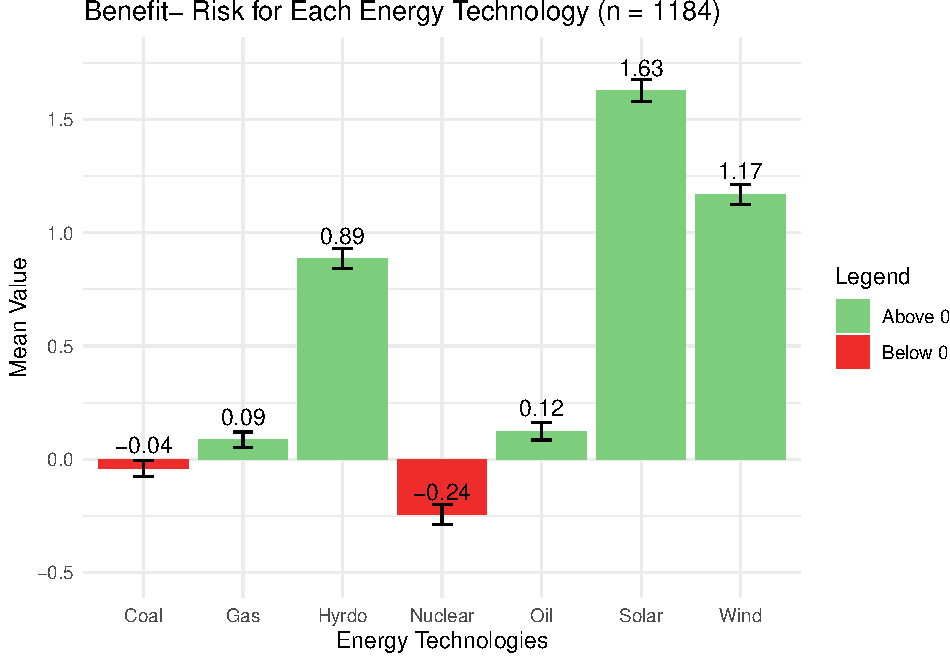
\includegraphics{nuclear-in-comparison_files/figure-latex/unnamed-chunk-10-1.pdf}

\newpage

\hypertarget{claim-1-demographic-variables-nuclear-solar-coal}{%
\section{Claim 1: Demographic variables: nuclear, solar,
coal}\label{claim-1-demographic-variables-nuclear-solar-coal}}

\begin{landscape}

\hypertarget{linear-regression-with-demographic-variables-caste-religion-gender-and-age}{%
\subsection{Linear Regression with demographic variables (caste,
religion, gender and
age)}\label{linear-regression-with-demographic-variables-caste-religion-gender-and-age}}

\begingroup\small\setlength{\tabcolsep}{1pt}\renewcommand{\arraystretch}{0.7}

\% Table created by stargazer v.5.2.3 by Marek Hlavac, Social Policy
Institute. E-mail: marek.hlavac at gmail.com \% Date and time: Sun, Mar
24, 2024 - 13:05:37

\begin{table}[!htbp] \centering 
  \caption{Linear Models: Perceived Risk and Net Perceived Benefit(Nuclear, Solar and Coal)} 
  \label{} 
\begin{tabular}{@{\extracolsep{5pt}}lcccccc} 
\\[-1.8ex]\hline 
\hline \\[-1.8ex] 
 & \multicolumn{6}{c}{\textit{Dependent variable:}} \\ 
\cline{2-7} 
\\[-1.8ex] & RiskNuclear & RiskSolar & RiskCoal & NetBenNuclear & NetBenSolar & NetBenCoal \\ 
\\[-1.8ex] & (1) & (2) & (3) & (4) & (5) & (6)\\ 
\hline \\[-1.8ex] 
 Uppercaste & 0.106 & $-$0.065 & 0.051 & $-$0.199$^{**}$ & $-$0.020 & $-$0.096 \\ 
  & (0.066) & (0.059) & (0.060) & (0.093) & (0.094) & (0.075) \\ 
  & & & & & & \\ 
 Male & 0.122$^{*}$ & $-$0.291$^{***}$ & 0.056 & $-$0.046 & 0.456$^{***}$ & $-$0.004 \\ 
  & (0.066) & (0.060) & (0.061) & (0.095) & (0.096) & (0.076) \\ 
  & & & & & & \\ 
 Hindu & $-$0.115 & $-$0.237$^{***}$ & 0.017 & 0.400$^{***}$ & 0.501$^{***}$ & 0.039 \\ 
  & (0.076) & (0.068) & (0.070) & (0.106) & (0.107) & (0.085) \\ 
  & & & & & & \\ 
 UrbanUrban & $-$0.099 & 0.521$^{***}$ & 0.110$^{*}$ & 0.390$^{***}$ & $-$0.711$^{***}$ & $-$0.015 \\ 
  & (0.065) & (0.058) & (0.059) & (0.092) & (0.093) & (0.073) \\ 
  & & & & & & \\ 
 age & 0.050$^{*}$ & $-$0.070$^{***}$ & 0.012 & $-$0.116$^{***}$ & 0.187$^{***}$ & $-$0.038 \\ 
  & (0.029) & (0.026) & (0.026) & (0.044) & (0.045) & (0.036) \\ 
  & & & & & & \\ 
 Constant & 3.309$^{***}$ & 2.325$^{***}$ & 3.005$^{***}$ & $-$0.355$^{**}$ & 0.835$^{***}$ & 0.059 \\ 
  & (0.108) & (0.097) & (0.099) & (0.154) & (0.156) & (0.124) \\ 
  & & & & & & \\ 
\hline \\[-1.8ex] 
Observations & 1,444 & 1,444 & 1,444 & 1,183 & 1,183 & 1,183 \\ 
R$^{2}$ & 0.012 & 0.100 & 0.003 & 0.041 & 0.122 & 0.003 \\ 
Adjusted R$^{2}$ & 0.009 & 0.097 & 0.00003 & 0.037 & 0.118 & $-$0.001 \\ 
Residual Std. Error & 1.176 (df = 1438) & 1.053 (df = 1438) & 1.080 (df = 1438) & 1.517 (df = 1177) & 1.533 (df = 1177) & 1.217 (df = 1177) \\ 
F Statistic & 3.552$^{***}$ (df = 5; 1438) & 31.870$^{***}$ (df = 5; 1438) & 1.010 (df = 5; 1438) & 10.122$^{***}$ (df = 5; 1177) & 32.725$^{***}$ (df = 5; 1177) & 0.705 (df = 5; 1177) \\ 
\hline 
\hline \\[-1.8ex] 
\textit{Note:}  & \multicolumn{6}{r}{$^{*}$p$<$0.1; $^{**}$p$<$0.05; $^{***}$p$<$0.01} \\ 
\end{tabular} 
\end{table} 
\endgroup

\end{landscape}

\begin{verbatim}
## 
## Regression Models Summary
## ================================================================================================================================================================
##                                                                                 Dependent variable:                                                             
##                     --------------------------------------------------------------------------------------------------------------------------------------------
##                           RiskNuclear              RiskSolar               RiskCoal            NetBenNuclear             NetBenSolar             NetBenCoal     
##                               (1)                     (2)                    (3)                    (4)                      (5)                    (6)         
## ----------------------------------------------------------------------------------------------------------------------------------------------------------------
## Uppercaste                   0.106                   -0.065                 0.051                 -0.199**                  -0.020                 -0.096       
##                             (0.066)                 (0.059)                (0.060)                (0.093)                  (0.094)                (0.075)       
##                                                                                                                                                                 
## Male                        0.122*                 -0.291***                0.056                  -0.046                  0.456***                -0.004       
##                             (0.066)                 (0.060)                (0.061)                (0.095)                  (0.096)                (0.076)       
##                                                                                                                                                                 
## Hindu                       -0.115                 -0.237***                0.017                 0.400***                 0.501***                0.039        
##                             (0.076)                 (0.068)                (0.070)                (0.106)                  (0.107)                (0.085)       
##                                                                                                                                                                 
## UrbanUrban                  -0.099                  0.521***                0.110*                0.390***                -0.711***                -0.015       
##                             (0.065)                 (0.058)                (0.059)                (0.092)                  (0.093)                (0.073)       
##                                                                                                                                                                 
## age                         0.050*                 -0.070***                0.012                -0.116***                 0.187***                -0.038       
##                             (0.029)                 (0.026)                (0.026)                (0.044)                  (0.045)                (0.036)       
##                                                                                                                                                                 
## Constant                   3.309***                 2.325***               3.005***               -0.355**                 0.835***                0.059        
##                             (0.108)                 (0.097)                (0.099)                (0.154)                  (0.156)                (0.124)       
##                                                                                                                                                                 
## ----------------------------------------------------------------------------------------------------------------------------------------------------------------
## Observations                 1,444                   1,444                  1,444                  1,183                    1,183                  1,183        
## R2                           0.012                   0.100                  0.003                  0.041                    0.122                  0.003        
## Adjusted R2                  0.009                   0.097                 0.00003                 0.037                    0.118                  -0.001       
## Residual Std. Error    1.176 (df = 1438)       1.053 (df = 1438)      1.080 (df = 1438)      1.517 (df = 1177)        1.533 (df = 1177)      1.217 (df = 1177)  
## F Statistic         3.552*** (df = 5; 1438) 31.870*** (df = 5; 1438) 1.010 (df = 5; 1438) 10.122*** (df = 5; 1177) 32.725*** (df = 5; 1177) 0.705 (df = 5; 1177)
## ================================================================================================================================================================
## Note:                                                                                                                                *p<0.1; **p<0.05; ***p<0.01
\end{verbatim}

\newpage

\hypertarget{claim-2-regional-differences}{%
\section{Claim 2: Regional
differences}\label{claim-2-regional-differences}}

We see huge differences for perceived risk and perceived benefit for
each technology from state to state. These graphs explore that. The
number of respondents from each state are also reported below.

\hypertarget{perceived-risk-by-state}{%
\subsection{Perceived risk by State}\label{perceived-risk-by-state}}

\begin{verbatim}
##   Maharashtra     Rajasthan    Tamil Nadu Uttar Pradesh   West Bengal 
##           653           677           320           125           386
\end{verbatim}

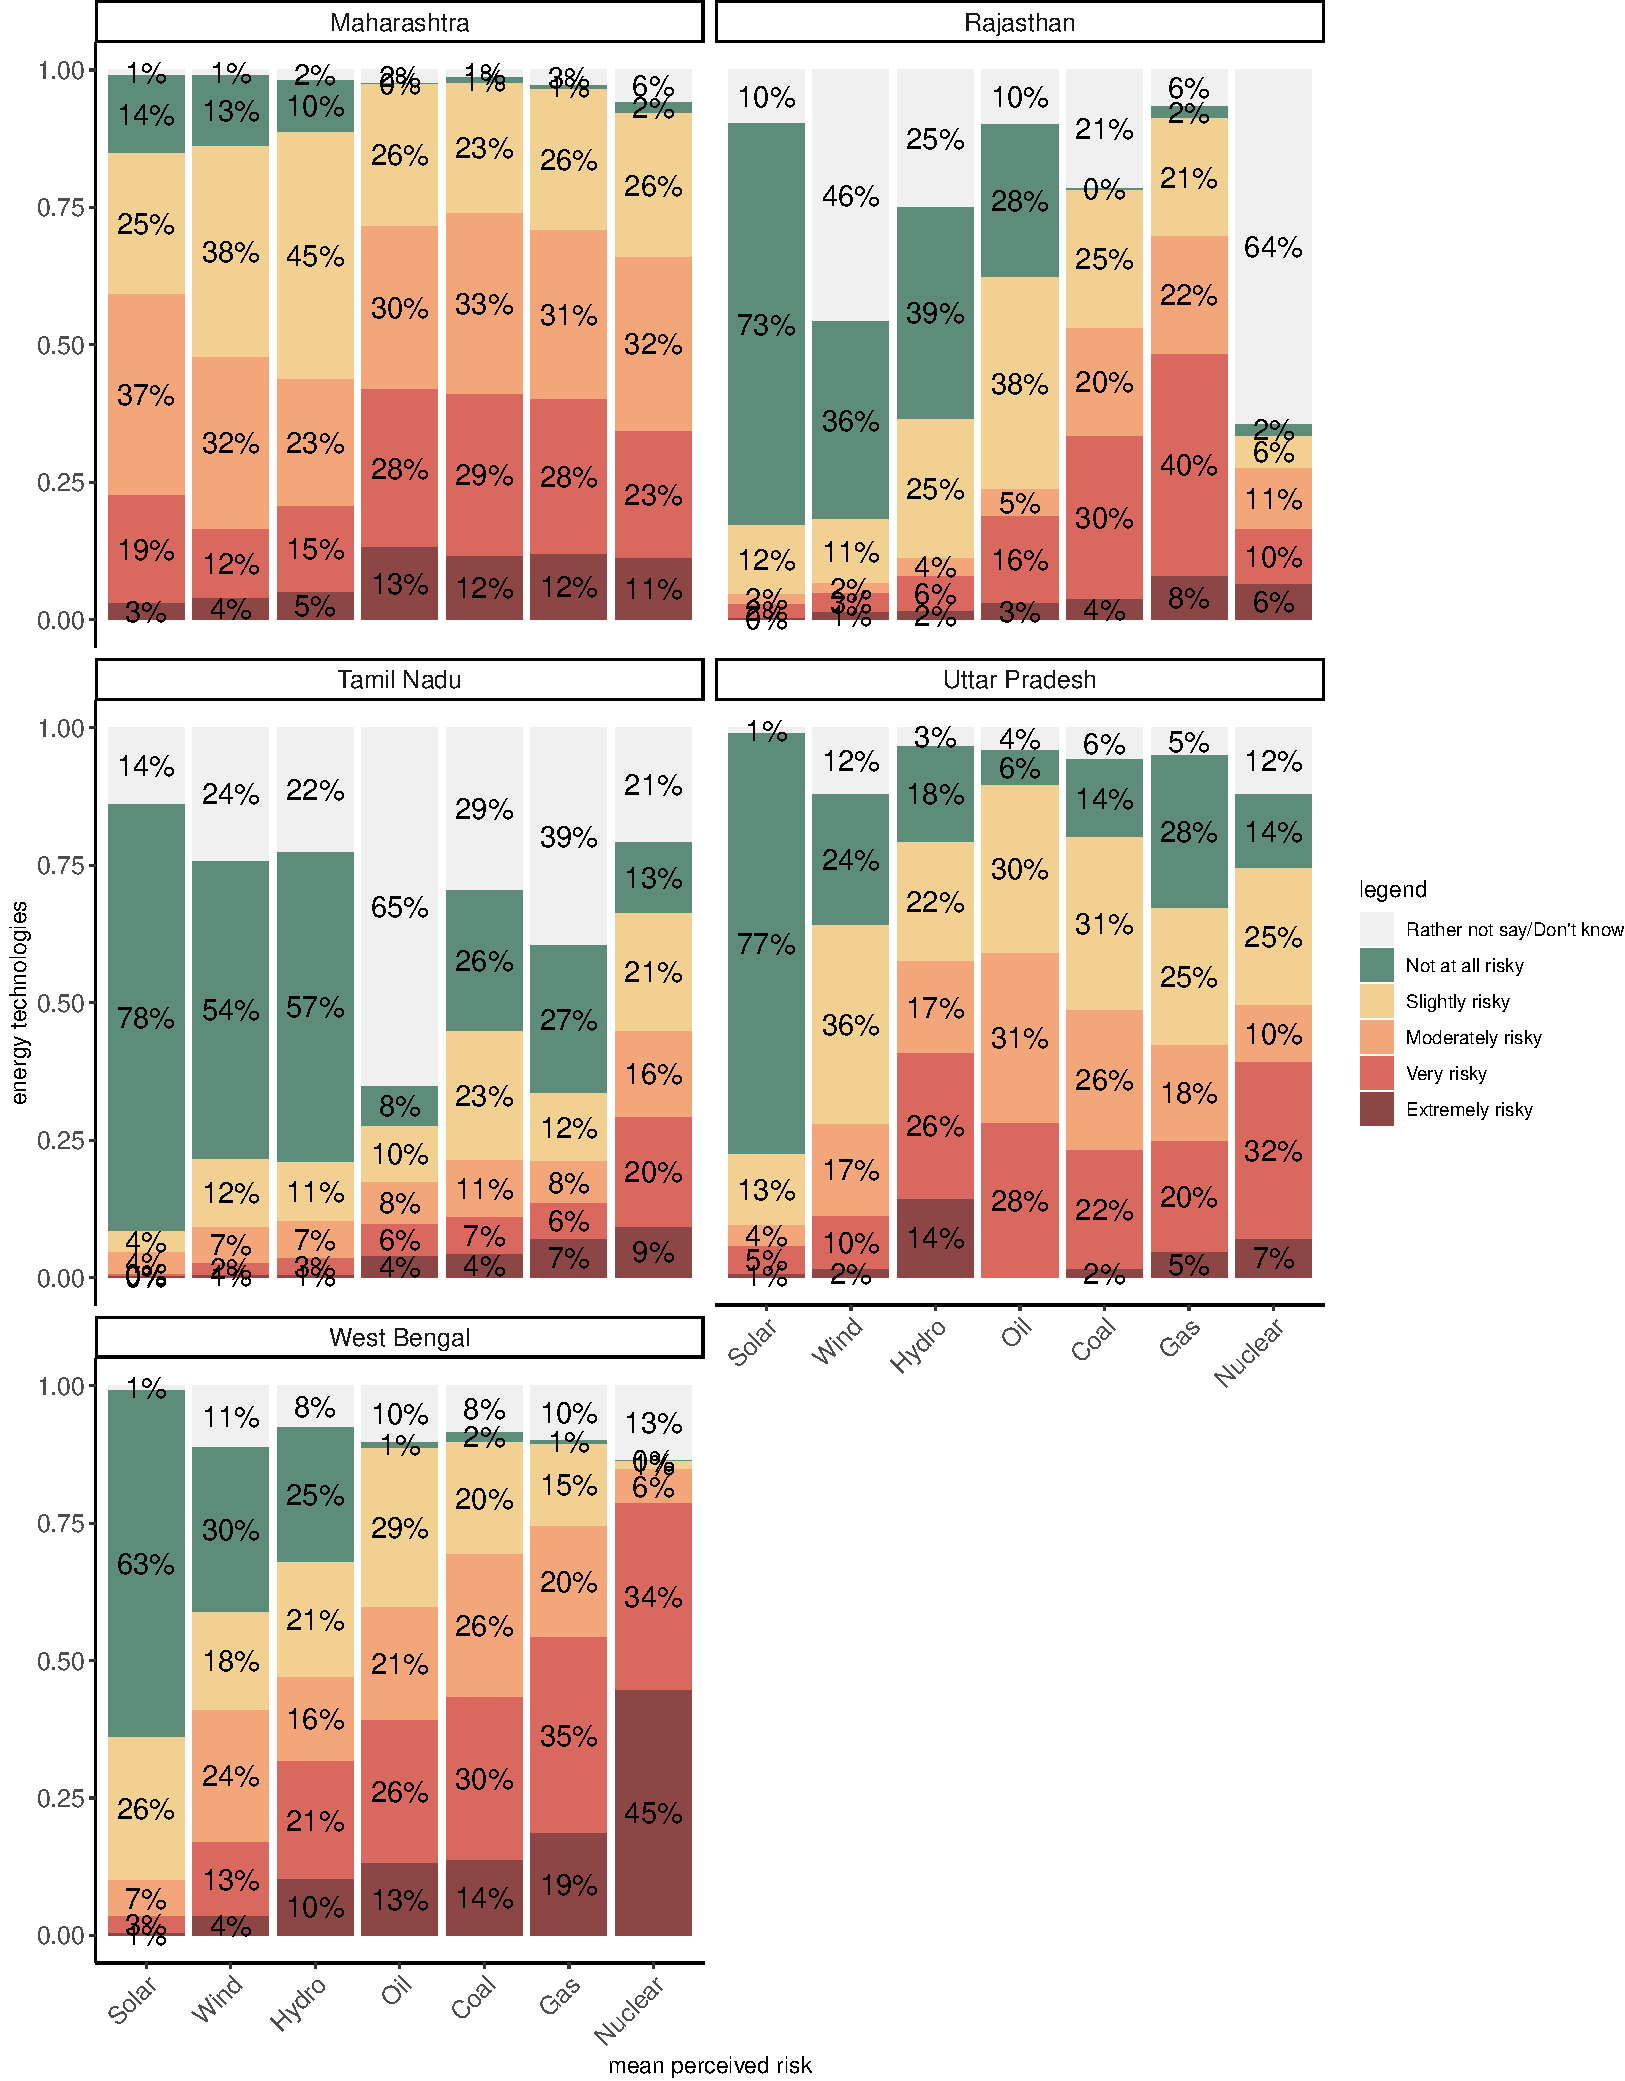
\includegraphics[width=0.8\linewidth,height=0.8\textheight]{nuclear-in-comparison_files/figure-latex/unnamed-chunk-15-1}

\newpage

\hypertarget{perceived-benefit-by-state}{%
\subsection{Perceived Benefit by
State}\label{perceived-benefit-by-state}}

\begin{verbatim}
##   Maharashtra     Rajasthan    Tamil Nadu Uttar Pradesh   West Bengal 
##           653           677           320           125           386
\end{verbatim}

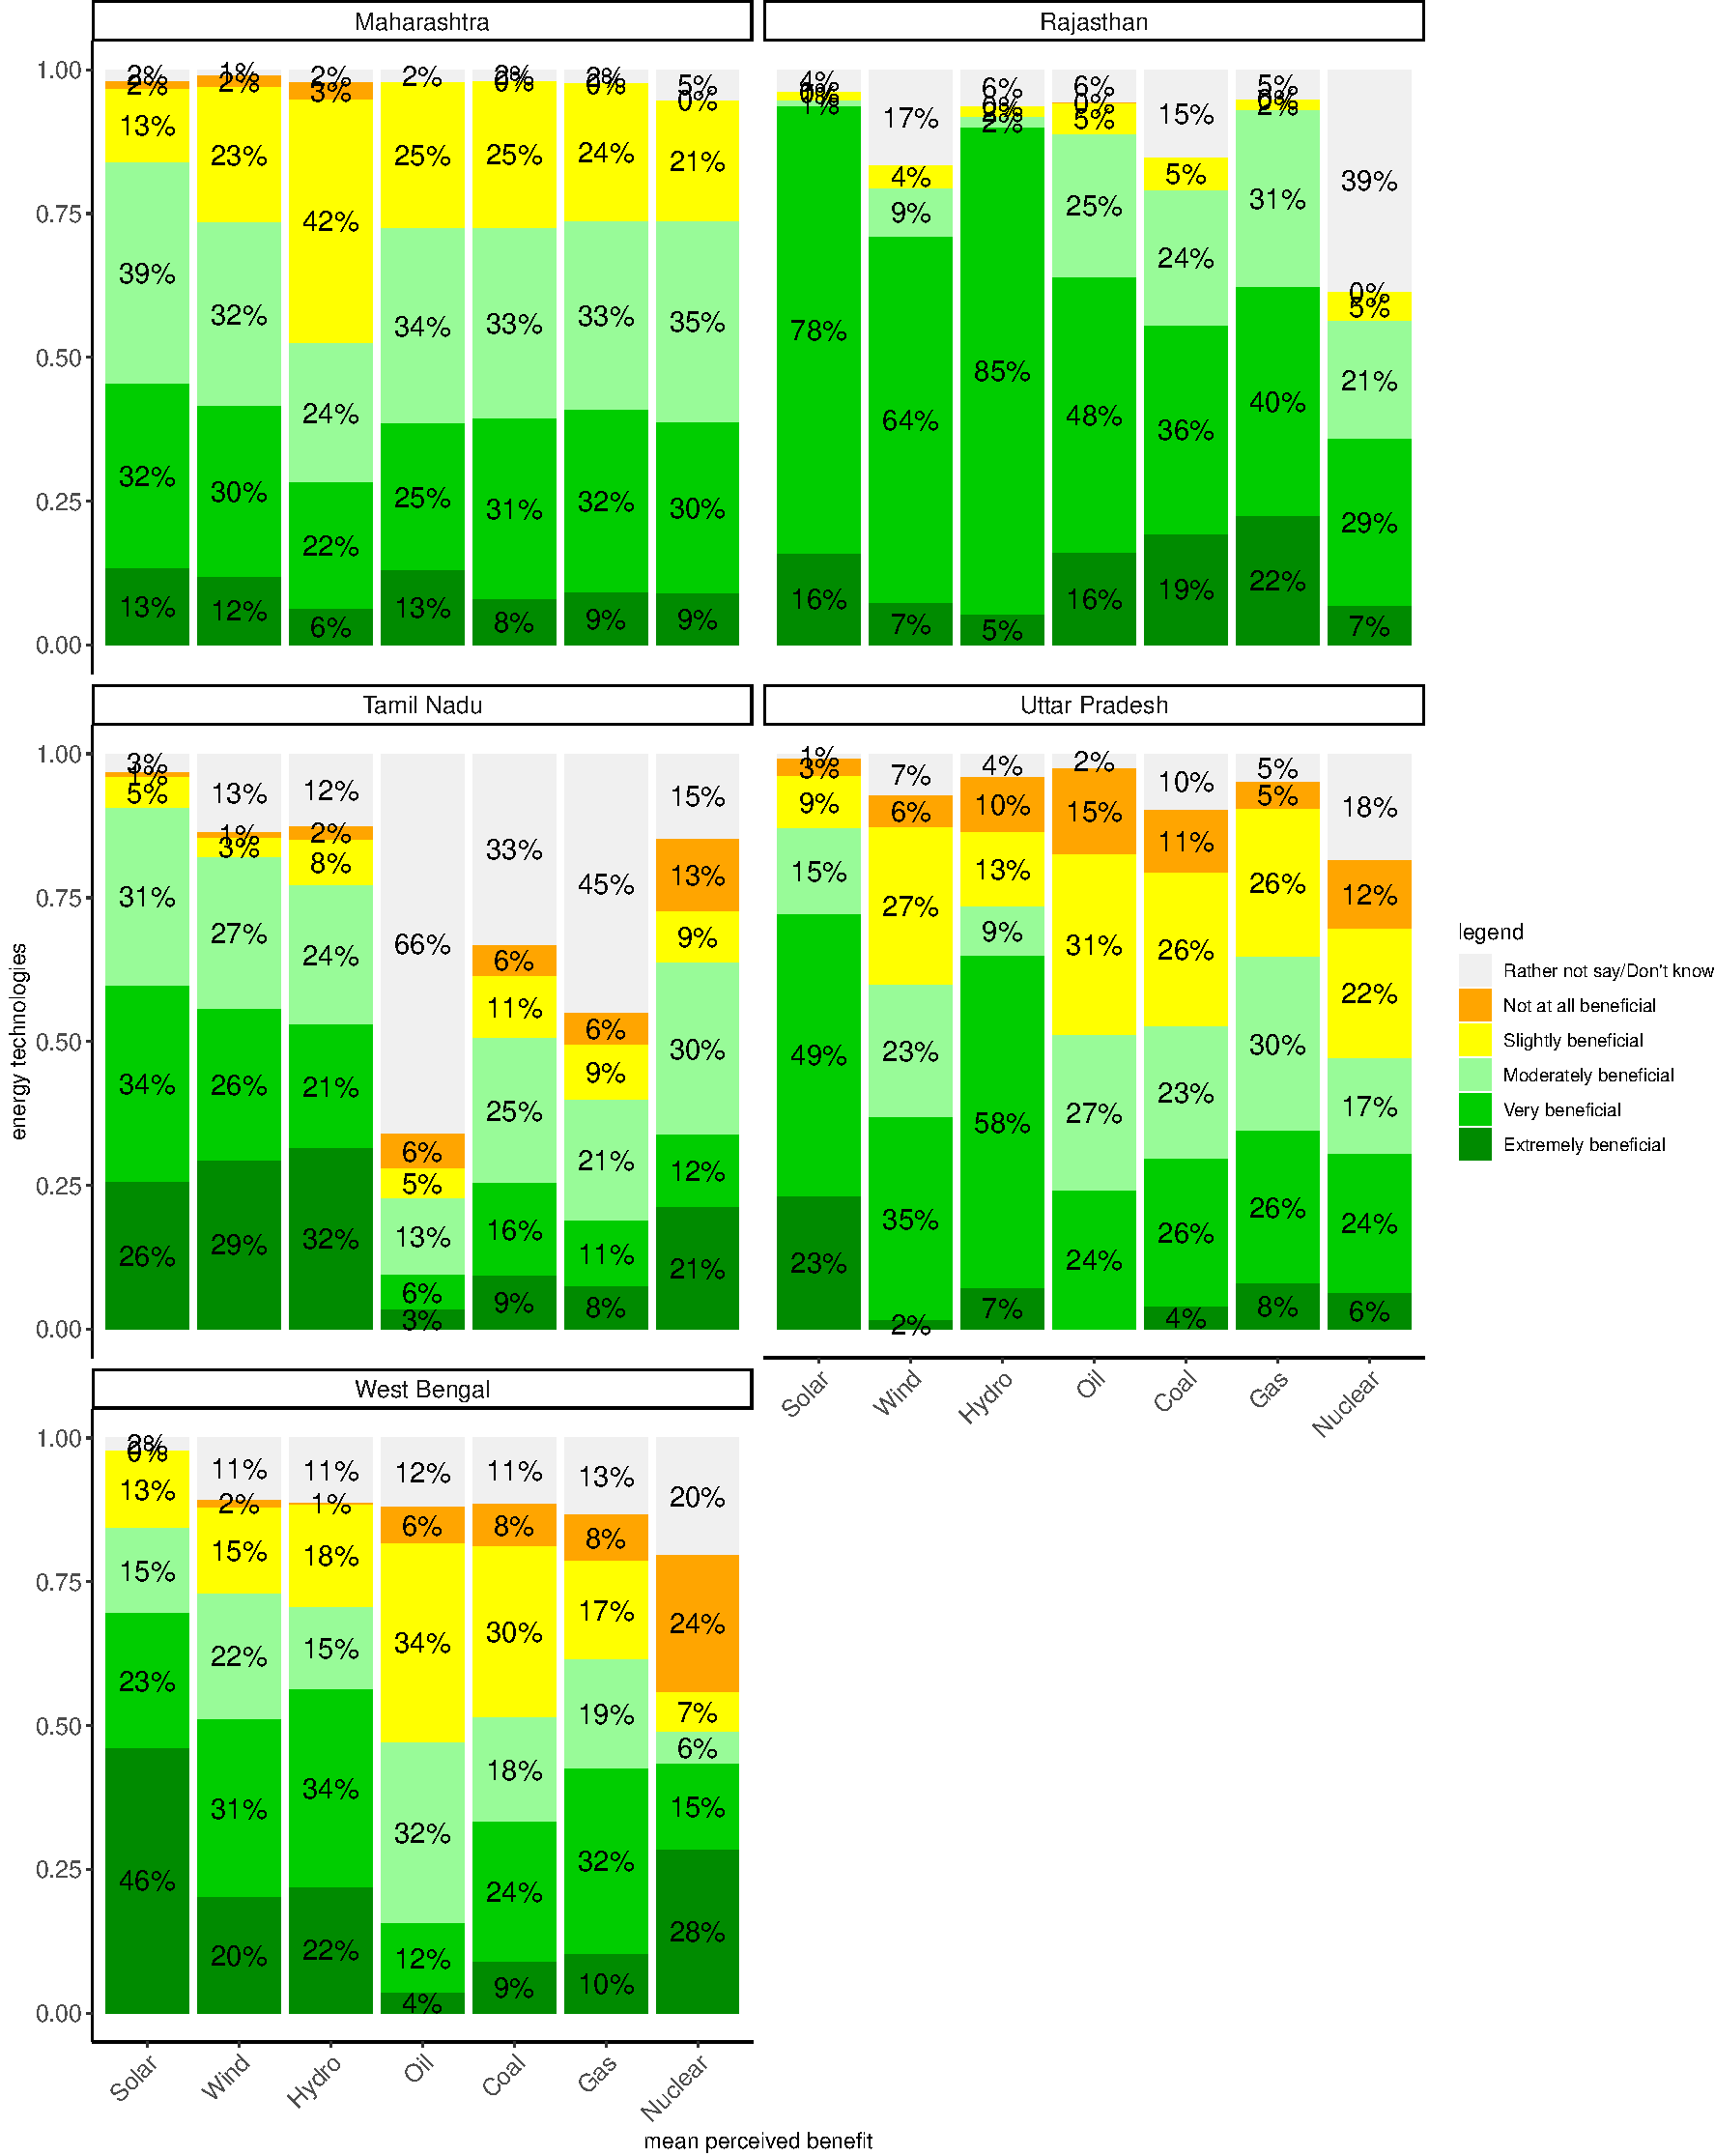
\includegraphics[width=1\linewidth,height=1\textheight]{nuclear-in-comparison_files/figure-latex/unnamed-chunk-16-1}
\#\# Radar chart - risk and benefit by state

\begin{verbatim}
## List of 5
##  $ Maharashtra  : tibble [14 x 6] (S3: tbl_df/tbl/data.frame)
##   ..$ State     : chr [1:14] "Maharashtra" "Maharashtra" "Maharashtra" "Maharashtra" ...
##   ..$ Tech      : Factor w/ 7 levels "Solar","Wind",..: 5 6 3 7 4 1 2 5 6 3 ...
##   ..$ Mean_Value: num [1:14] 3.27 3.25 2.61 3.16 3.29 ...
##   ..$ sd        : num [1:14] 0.992 1.01 1.032 1.033 1.014 ...
##   ..$ se        : num [1:14] 0.0388 0.0395 0.0404 0.0404 0.0397 ...
##   ..$ Category  : chr [1:14] "Risky" "Risky" "Risky" "Risky" ...
##  $ Rajasthan    : tibble [14 x 6] (S3: tbl_df/tbl/data.frame)
##   ..$ State     : chr [1:14] "Rajasthan" "Rajasthan" "Rajasthan" "Rajasthan" ...
##   ..$ Tech      : Factor w/ 7 levels "Solar","Wind",..: 5 6 3 7 4 1 2 5 6 3 ...
##   ..$ Mean_Value: num [1:14] 3.14 3.33 1.76 3.35 2.19 ...
##   ..$ sd        : num [1:14] 0.945 1.001 1.016 1.144 1.155 ...
##   ..$ se        : num [1:14] 0.0363 0.0385 0.039 0.0439 0.0444 ...
##   ..$ Category  : chr [1:14] "Risky" "Risky" "Risky" "Risky" ...
##  $ Tamil Nadu   : tibble [14 x 6] (S3: tbl_df/tbl/data.frame)
##   ..$ State     : chr [1:14] "Tamil Nadu" "Tamil Nadu" "Tamil Nadu" "Tamil Nadu" ...
##   ..$ Tech      : Factor w/ 7 levels "Solar","Wind",..: 5 6 3 7 4 1 2 5 6 3 ...
##   ..$ Mean_Value: num [1:14] 2.15 2.24 1.46 2.89 2.68 ...
##   ..$ sd        : num [1:14] 1.196 1.417 0.862 1.282 1.296 ...
##   ..$ se        : num [1:14] 0.0668 0.0792 0.0482 0.0717 0.0724 ...
##   ..$ Category  : chr [1:14] "Risky" "Risky" "Risky" "Risky" ...
##  $ Uttar Pradesh: tibble [14 x 6] (S3: tbl_df/tbl/data.frame)
##   ..$ State     : chr [1:14] "Uttar Pradesh" "Uttar Pradesh" "Uttar Pradesh" "Uttar Pradesh" ...
##   ..$ Tech      : Factor w/ 7 levels "Solar","Wind",..: 5 6 3 7 4 1 2 5 6 3 ...
##   ..$ Mean_Value: num [1:14] 2.63 2.46 2.98 2.94 2.84 ...
##   ..$ sd        : num [1:14] 1.052 1.254 1.354 1.265 0.926 ...
##   ..$ se        : num [1:14] 0.0941 0.1122 0.1211 0.1132 0.0828 ...
##   ..$ Category  : chr [1:14] "Risky" "Risky" "Risky" "Risky" ...
##  $ West Bengal  : tibble [14 x 6] (S3: tbl_df/tbl/data.frame)
##   ..$ State     : chr [1:14] "West Bengal" "West Bengal" "West Bengal" "West Bengal" ...
##   ..$ Tech      : Factor w/ 7 levels "Solar","Wind",..: 5 6 3 7 4 1 2 5 6 3 ...
##   ..$ Mean_Value: num [1:14] 3.36 3.63 2.7 4.4 3.23 ...
##   ..$ sd        : num [1:14] 1.05 1.01 1.37 0.72 1.1 ...
##   ..$ se        : num [1:14] 0.0536 0.0517 0.0698 0.0366 0.0558 ...
##   ..$ Category  : chr [1:14] "Risky" "Risky" "Risky" "Risky" ...
\end{verbatim}

\begin{verbatim}
## 'data.frame':    2161 obs. of  193 variables:
##  $ Respondent          : int  1 2 3 4 5 6 7 8 9 10 ...
##  $ Language            : chr  "HI" "BN" "BN" "BN" ...
##  $ Survey_Date         : chr  "05-12-2021" "08-12-2021" "08-12-2021" "08-12-2021" ...
##  $ State               : chr  "Uttar Pradesh" "West Bengal" "West Bengal" "West Bengal" ...
##  $ Risky_Hydro         : num  3 1 2 2 4 2 2 NA 3 5 ...
##  $ Risky_Solar         : num  1 1 1 2 1 1 1 2 3 1 ...
##  $ Risky_Wind          : num  1 2 2 2 1 1 1 1 2 3 ...
##  $ Risky_Nuclear       : num  2 4 4 4 5 3 2 4 5 NA ...
##  $ Risky_Coal          : num  3 4 NA 4 5 2 3 2 4 3 ...
##  $ Risky_Gas           : num  3 4 4 3 4 1 3 3 4 5 ...
##  $ Risky_Oil           : num  3 3 2 3 4 2 3 3 4 2 ...
##  $ Risky_INDHydro      : num  3 3 2 2 2 2 2 3 4 5 ...
##  $ Risky_INDSolar      : num  3 1 1 1 5 2 2 3 1 1 ...
##  $ Risky_INDWind       : num  NA 4 5 2 1 NA 3 NA 3 3 ...
##  $ Risky_INDBiogas     : num  3 1 NA 2 2 2 2 NA 3 4 ...
##  $ Risky_INDDiesel     : num  3 2 2 2 4 4 4 2 3 4 ...
##  $ Risky_INDKerosene   : num  NA 1 2 1 3 2 4 2 4 5 ...
##  $ Risky_INDFirewoodetc: num  2 2 1 1 2 1 1 1 3 5 ...
##  $ Risky_INDLPG        : num  5 3 1 1 5 2 2 4 5 5 ...
##  $ Ben_Hydro           : num  4 3 2 2 4 2 2 NA 2 4 ...
##  $ Ben_Solar           : num  4 4 2 3 3 3 3 4 3 3 ...
##  $ Ben_Wind            : num  3 4 2 2 5 1 2 2 5 3 ...
##  $ Ben_Nuclear         : num  5 2 NA 1 1 1 1 4 3 5 ...
##  $ Ben_Coal            : num  5 4 2 1 1 1 1 NA 4 4 ...
##  $ Ben_Gas             : num  1 4 2 1 4 2 1 5 4 4 ...
##  $ Ben_Oil             : num  3 3 2 2 3 1 2 3 5 3 ...
##  $ Ben_INDHydro        : num  5 3 2 2 4 3 2 NA 3 NA ...
##  $ Ben_INDSolar        : num  3 2 NA NA 2 2 1 4 2 5 ...
##  $ Ben_INDWind         : num  2 NA NA 2 2 NA 2 NA 3 3 ...
##  $ Ben_INDDiesel       : num  1 3 2 2 3 1 1 2 3 4 ...
##  $ Ben_INDBiogas       : num  5 NA 2 2 4 3 1 2 5 4 ...
##  $ Ben_INDFirewoodetc  : num  4 3 3 3 1 3 2 2 4 1 ...
##  $ Ben_INDLPG          : num  2 2 3 2 5 2 3 NA NA 1 ...
##  $ Ben_INDKerosene     : num  2 2 3 2 1 2 2 2 NA 2 ...
##  $ N_accept            : num  3 1 1 1 1 2 2 NA NA NA ...
##  $ N_reluctantlyaccept : num  1 2 2 2 NA 2 2 NA NA NA ...
##  $ N_reject            : num  3 NA NA 4 NA 4 4 NA NA NA ...
##  $ K_IINTRFER          : num  4 4 2 5 4 2 3 2 3 1 ...
##  $ K_IPRIVACY          : num  2 NA 2 2 3 3 3 2 4 5 ...
##  $ K_SHARM             : num  5 NA 2 4 5 3 3 1 3 5 ...
##  $ K_IPROTECT          : num  3 4 3 2 1 3 NA 2 3 1 ...
##  $ K_SLIMCHOI          : num  1 5 NA NA 5 NA NA NA 3 5 ...
##  $ K_SPROTECT          : num  2 4 NA NA 3 3 3 2 4 5 ...
##  $ K_HEQUAL            : num  1 2 4 4 4 2 2 5 4 5 ...
##  $ K_HREVDIS1          : num  5 3 3 2 2 3 3 4 4 4 ...
##  $ K_EDISCRIM          : num  NA NA 3 2 4 3 3 NA 5 3 ...
##  $ K_ERADEQ1           : num  5 5 5 5 5 5 1 4 NA 4 ...
##  $ K_EWEALTH           : num  4 NA NA 3 5 3 3 5 NA 4 ...
##  $ K_ERADEQ2           : num  5 5 5 5 1 5 5 5 4 5 ...
##  $ DECISIONDECEN       : num  5 NA NA NA NA 3 3 NA 3 NA ...
##  $ DECISIONCEN         : num  3 3 NA NA NA NA 3 4 NA 4 ...
##  $ SYSTEMTOTAL         : num  1 5 5 3 2 3 3 5 NA 5 ...
##  $ SYSTEMTECHNO        : num  2 NA 3 3 NA 5 NA 4 5 4 ...
##  $ SYSTEMDEMO          : num  2 3 NA NA 5 3 NA 3 3 5 ...
##  $ SYSTEMRELIGION      : num  1 NA NA 3 4 NA NA 3 4 5 ...
##  $ INDUSTRYSMALL       : num  5 5 2 2 5 2 2 4 5 5 ...
##  $ INDUSTRYLARGE       : num  3 4 4 5 5 5 5 5 5 5 ...
##  $ ECONOMYLOCAL        : num  1 2 4 2 1 3 4 4 4 3 ...
##  $ ECONOMYGLOBAL       : num  1 3 3 4 4 NA 1 5 4 4 ...
##  $ DEVOVERENV          : num  1 3 3 NA NA 3 3 4 4 3 ...
##  $ ENVOVERDEV          : num  2 NA NA NA 2 NA 3 4 5 5 ...
##  $ OWNERPVT            : num  4 4 4 3 3 3 NA 1 NA 4 ...
##  $ OWNERPUB            : num  3 NA 2 3 2 2 NA 2 NA 2 ...
##  $ OWNERREG            : num  1 NA 3 5 NA 3 3 5 NA 4 ...
##  $ OWNERNOREG          : num  4 NA NA 3 NA NA 3 5 NA 3 ...
##  $ WEALTHLIM           : num  3 4 3 3 4 NA NA 4 NA 5 ...
##  $ MECHANISATION       : num  4 5 5 5 5 4 5 4 4 5 ...
##  $ DISPLACESOLAR       : num  4 1 1 2 1 2 2 2 2 1 ...
##  $ POLLUTESOLAR        : num  4 1 1 2 1 1 1 1 1 1 ...
##  $ HEALTHSOLAR         : num  NA 2 2 2 1 2 1 1 1 1 ...
##  $ JOBSSOLAR           : num  NA 2 NA NA 1 NA NA 1 3 2 ...
##  $ BEAUTYSOLAR         : num  NA 2 2 1 1 2 1 1 1 1 ...
##  $ PRIDESOLAR          : num  NA 4 2 4 5 2 4 5 4 5 ...
##  $ NPRIDESOLAR         : num  3 4 2 4 4 3 4 5 5 5 ...
##  $ DEVSOLAR            : num  2 2 3 2 5 3 4 5 4 5 ...
##  $ PROSPERSOLAR        : num  2 2 3 3 2 2 3 2 1 4 ...
##  $ RELYSOLAR           : num  4 2 NA 3 NA 3 NA 5 2 4 ...
##  $ DISPLACEROOFS       : num  3 2 2 2 1 2 2 1 2 1 ...
##  $ POLLUTEROOFS        : num  1 2 2 1 1 2 2 1 1 1 ...
##  $ HEALTHROOFS         : num  1 1 2 1 1 2 2 1 1 1 ...
##  $ JOBSROOFS           : num  2 NA NA 3 1 NA NA 1 NA 4 ...
##  $ BEAUTYROOFS         : num  4 2 1 2 1 1 2 1 1 1 ...
##  $ PRIDEROOFS          : num  2 2 2 2 5 3 3 5 4 5 ...
##  $ NPRIDEROOFS         : num  1 NA 2 3 5 3 3 5 NA 5 ...
##  $ DEVROOFS            : num  2 2 2 NA 5 2 4 5 NA 5 ...
##  $ PROSPERROOFS        : num  3 3 1 2 3 3 4 5 NA 5 ...
##  $ RELYROOFS           : num  3 3 3 2 NA 4 4 5 3 4 ...
##  $ DISPLACEDIESEL      : num  1 4 2 2 1 2 4 NA 4 2 ...
##  $ POLLUTEDIESEL       : num  4 2 4 3 1 4 2 5 5 4 ...
##  $ HEALTHDIESEL        : num  NA 3 4 3 2 3 3 4 4 1 ...
##  $ JOBSDIESEL          : num  3 NA NA 4 NA 3 3 1 3 4 ...
##  $ BEAUTYDIESEL        : num  3 4 5 3 2 4 5 4 5 4 ...
##  $ PRIDEDIESEL         : num  2 3 3 2 NA 2 2 4 2 4 ...
##  $ NPRIDEDIESEL        : num  3 3 4 1 1 2 3 4 NA 4 ...
##  $ DEVDIESEL           : num  2 NA 3 1 1 2 NA 2 NA 4 ...
##  $ PROSPERDIESEL       : num  4 3 3 2 1 4 5 3 5 5 ...
##  $ RELYDIESEL          : num  1 3 4 2 NA 3 NA 4 NA 4 ...
##  $ DISPLACEFIRE        : num  4 1 2 2 4 4 3 2 2 4 ...
##  $ POLLUTEFIRE         : num  2 1 1 2 3 2 1 3 2 4 ...
##   [list output truncated]
\end{verbatim}

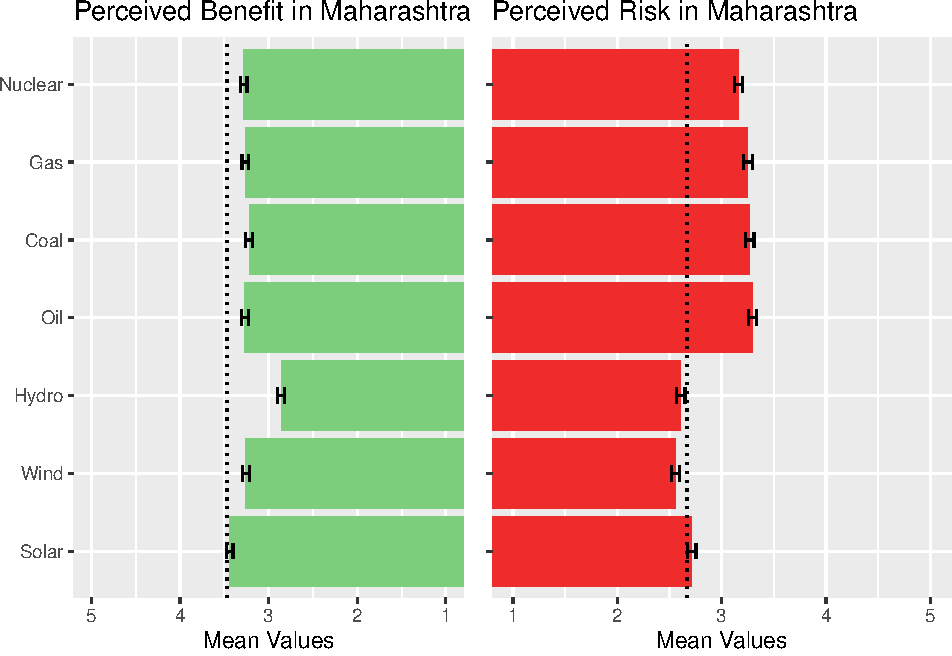
\includegraphics{nuclear-in-comparison_files/figure-latex/unnamed-chunk-18-1.pdf}
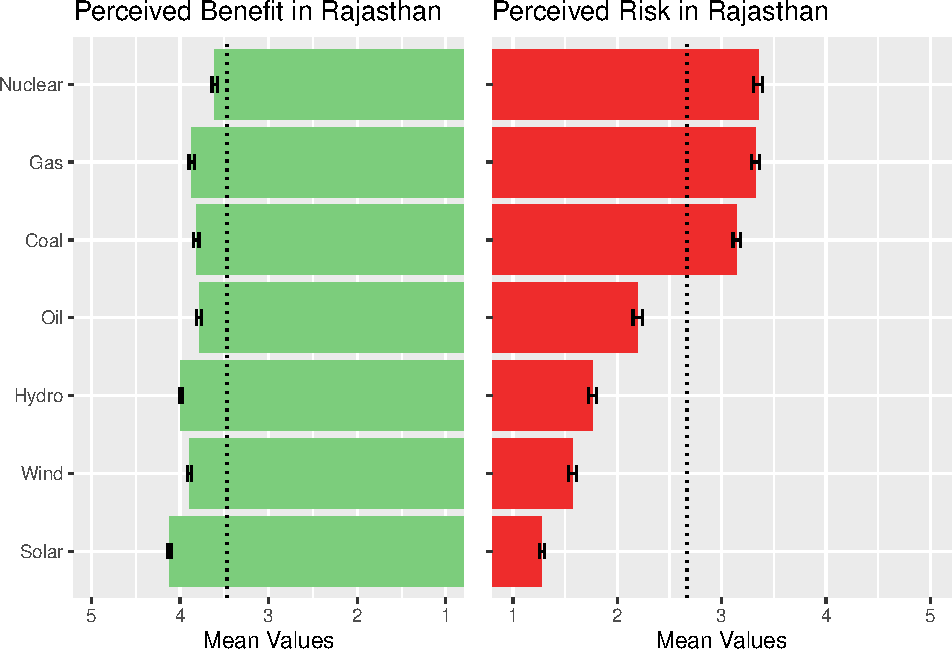
\includegraphics{nuclear-in-comparison_files/figure-latex/unnamed-chunk-18-2.pdf}
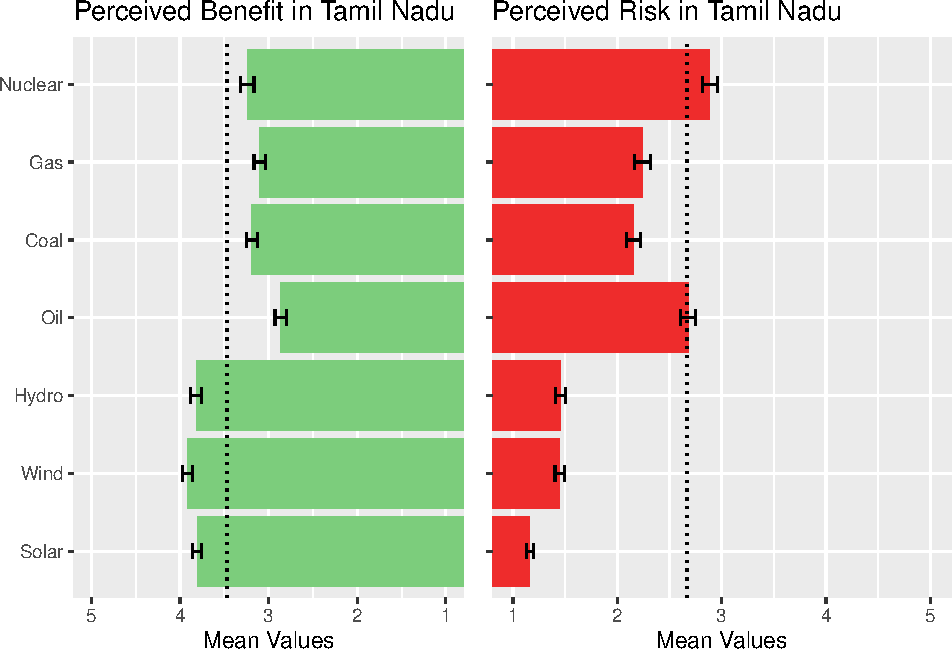
\includegraphics{nuclear-in-comparison_files/figure-latex/unnamed-chunk-18-3.pdf}
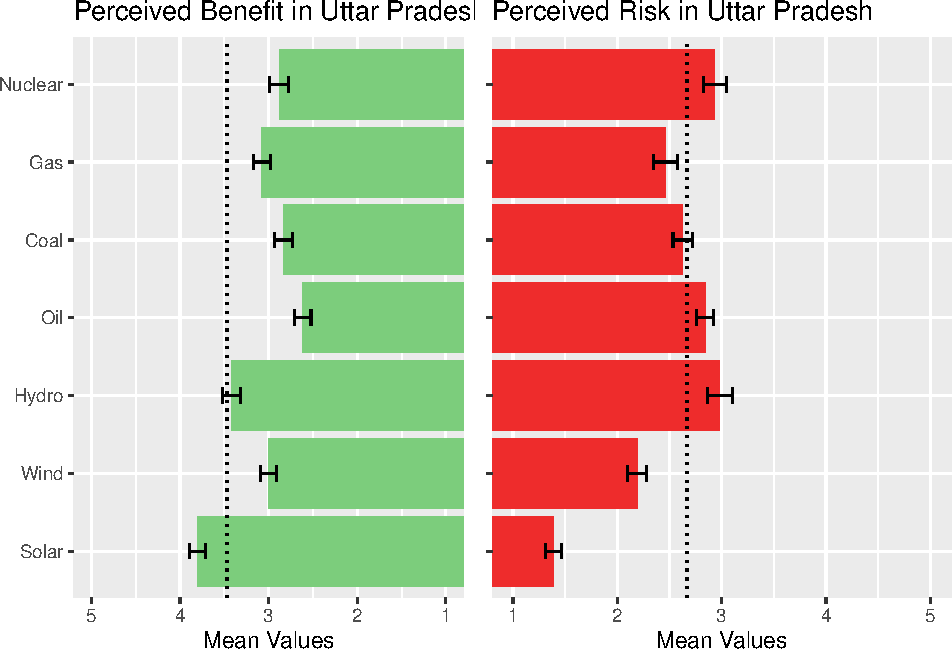
\includegraphics{nuclear-in-comparison_files/figure-latex/unnamed-chunk-18-4.pdf}
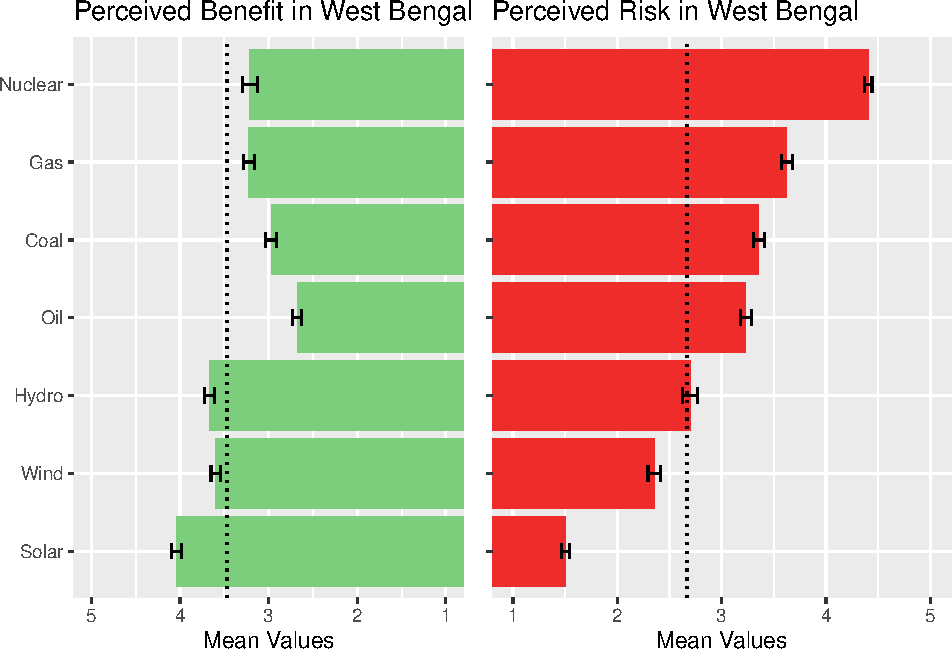
\includegraphics{nuclear-in-comparison_files/figure-latex/unnamed-chunk-18-5.pdf}

\hypertarget{maharshtra-t-tests}{%
\section{Maharshtra t tests}\label{maharshtra-t-tests}}

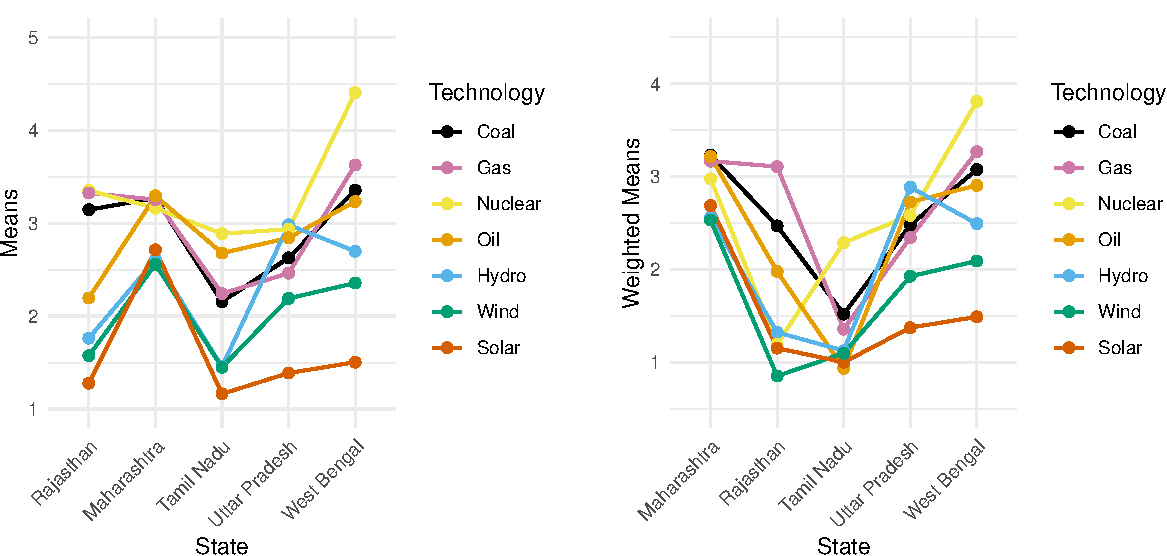
\includegraphics{nuclear-in-comparison_files/figure-latex/unnamed-chunk-19-1.pdf}

\hypertarget{tamil-nadu-t-tests}{%
\section{Tamil Nadu t tests}\label{tamil-nadu-t-tests}}

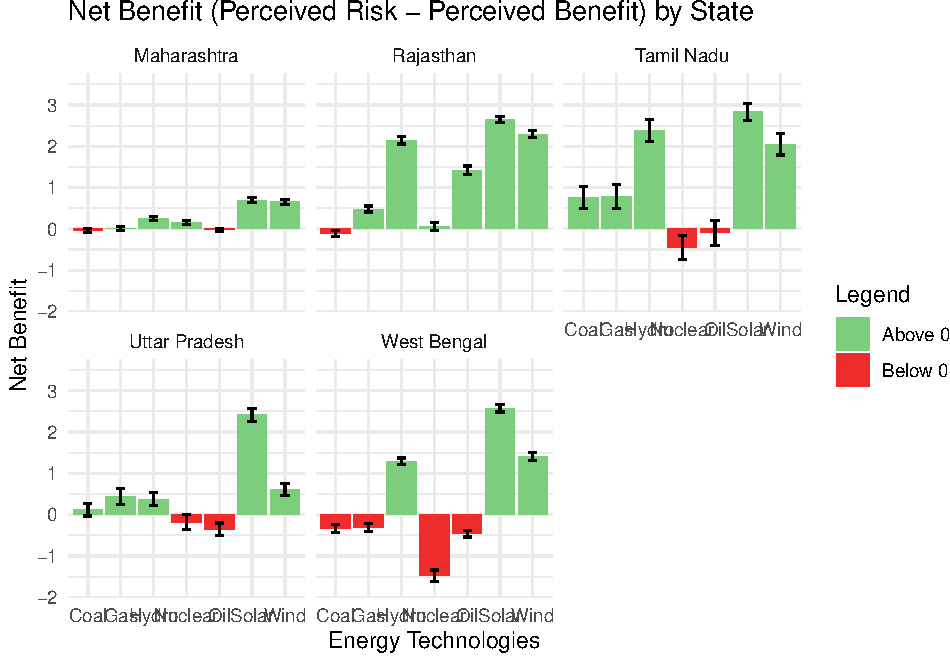
\includegraphics{nuclear-in-comparison_files/figure-latex/unnamed-chunk-20-1.pdf}

\hypertarget{uttar-pradesh-t-tests}{%
\section{Uttar Pradesh t tests}\label{uttar-pradesh-t-tests}}

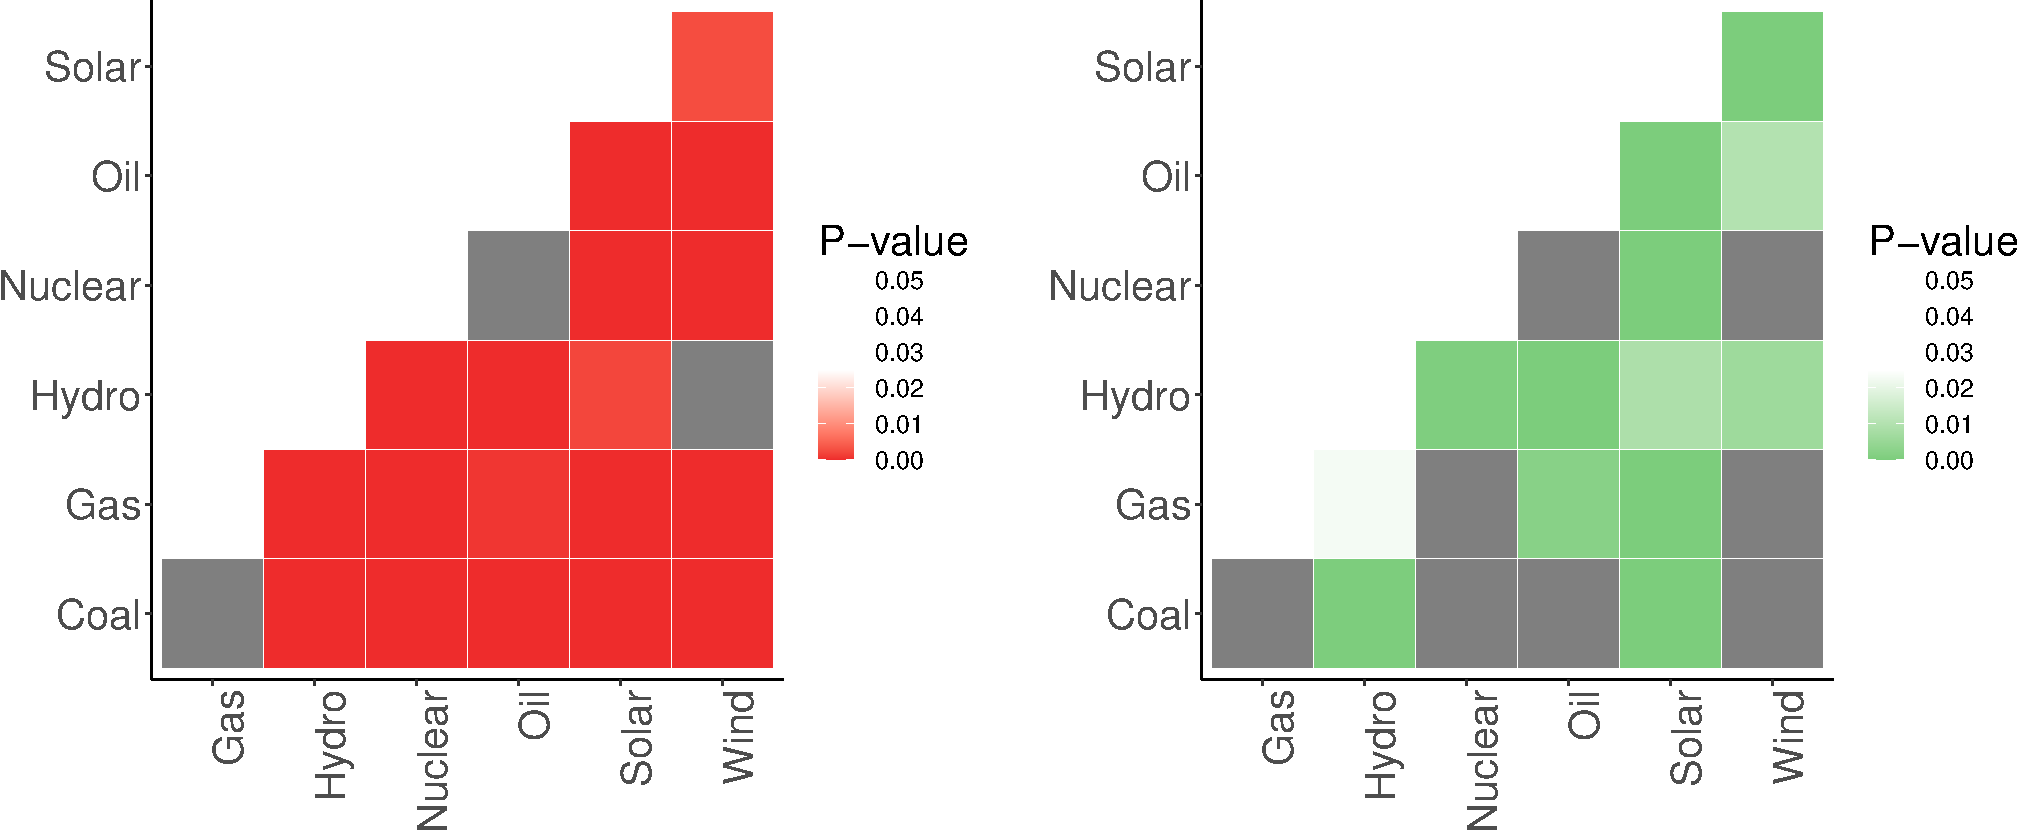
\includegraphics{nuclear-in-comparison_files/figure-latex/unnamed-chunk-21-1.pdf}

\hypertarget{rajasthan-t-tests}{%
\section{Rajasthan t tests}\label{rajasthan-t-tests}}

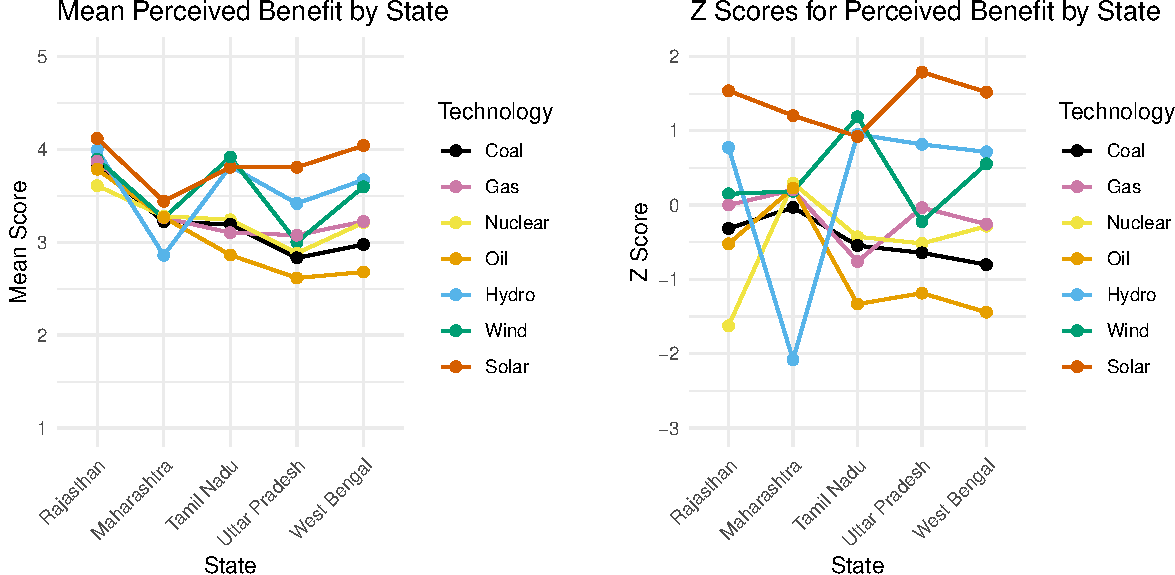
\includegraphics{nuclear-in-comparison_files/figure-latex/unnamed-chunk-22-1.pdf}

\hypertarget{west-bengal-t-tests}{%
\section{West Bengal t tests}\label{west-bengal-t-tests}}

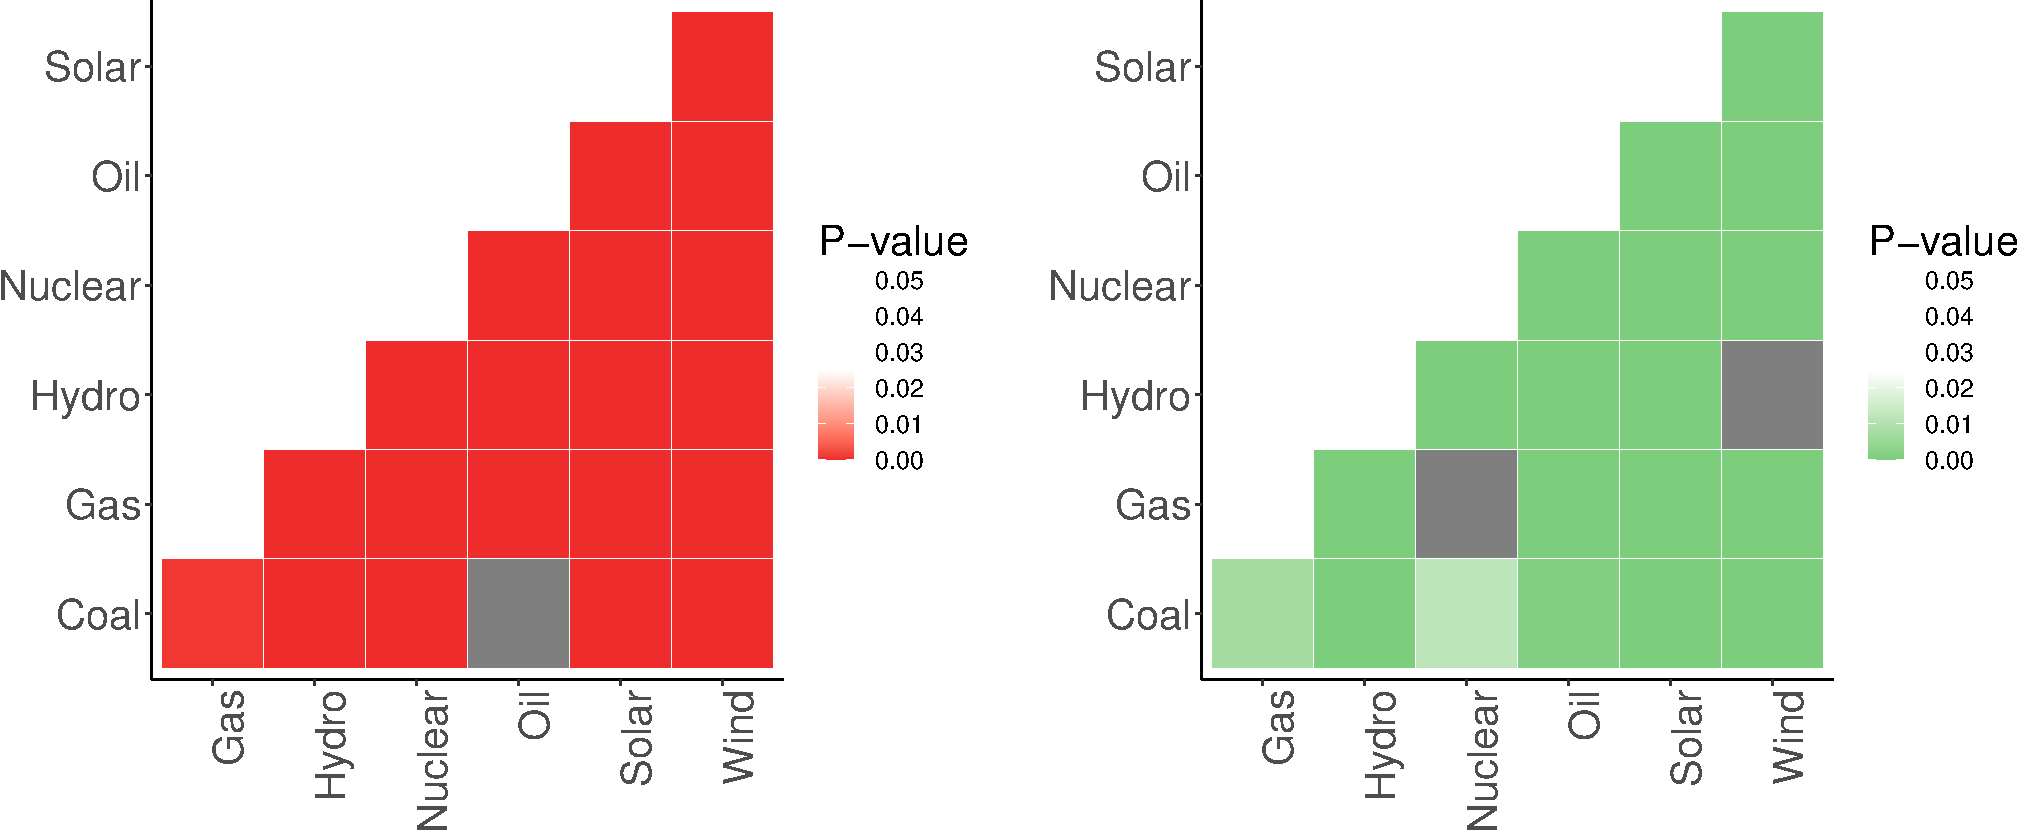
\includegraphics{nuclear-in-comparison_files/figure-latex/unnamed-chunk-23-1.pdf}
\#\# Net benefit by state

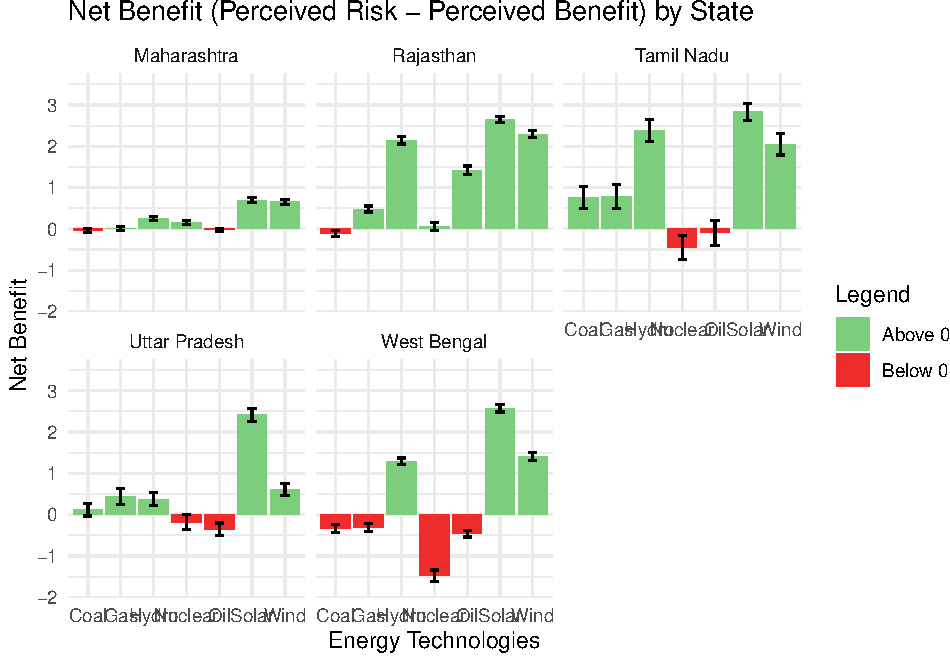
\includegraphics{nuclear-in-comparison_files/figure-latex/unnamed-chunk-25-1.pdf}

\newpage

\hypertarget{mean-perceived-risk-and-weighted-mean}{%
\subsection{Mean Perceived Risk and Weighted
Mean}\label{mean-perceived-risk-and-weighted-mean}}

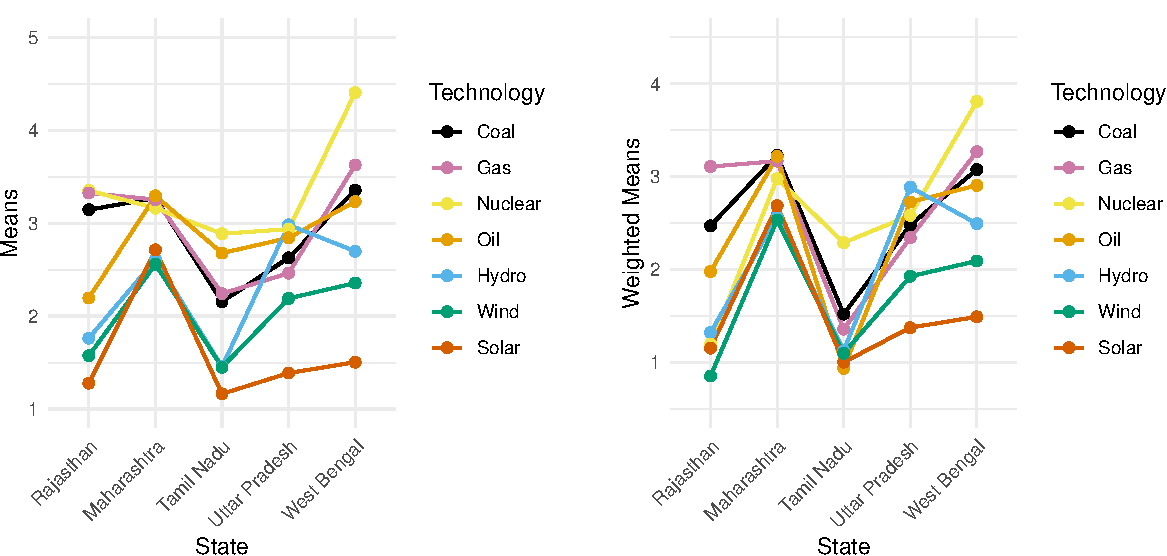
\includegraphics[width=1\linewidth,height=1\textheight]{nuclear-in-comparison_files/figure-latex/unnamed-chunk-29-1}

\newpage

\hypertarget{mean-perceived-risk-and-weighten-means-by-technologies--solar-coal-and-nuclear}{%
\subsection{Mean Perceived risk and weighten means by Technologies-
solar, coal and
nuclear}\label{mean-perceived-risk-and-weighten-means-by-technologies--solar-coal-and-nuclear}}

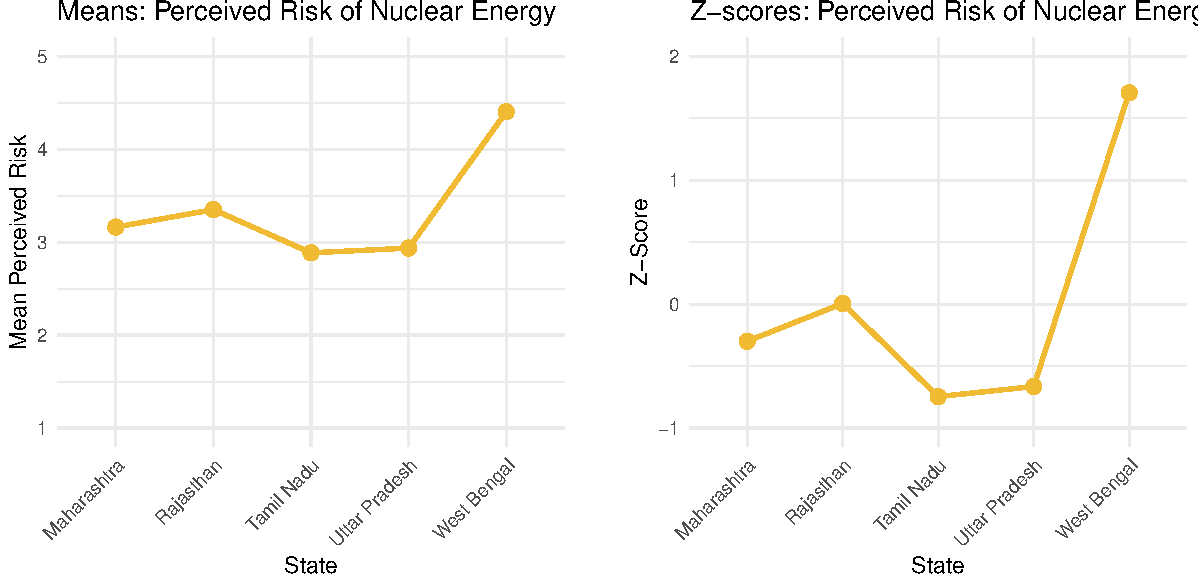
\includegraphics[width=1\linewidth,height=1\textheight]{nuclear-in-comparison_files/figure-latex/unnamed-chunk-33-1}

\hypertarget{zscores---3-techs---solar-nuclear-and-coal}{%
\subsection{Zscores - 3 techs - solar, nuclear and
coal}\label{zscores---3-techs---solar-nuclear-and-coal}}

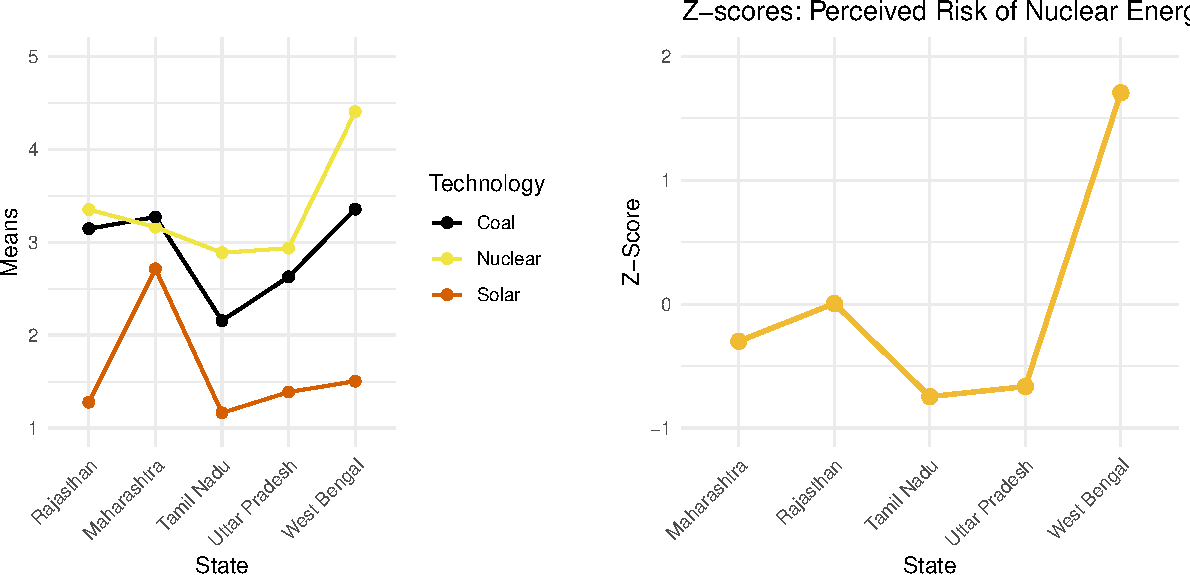
\includegraphics{nuclear-in-comparison_files/figure-latex/unnamed-chunk-34-1.pdf}
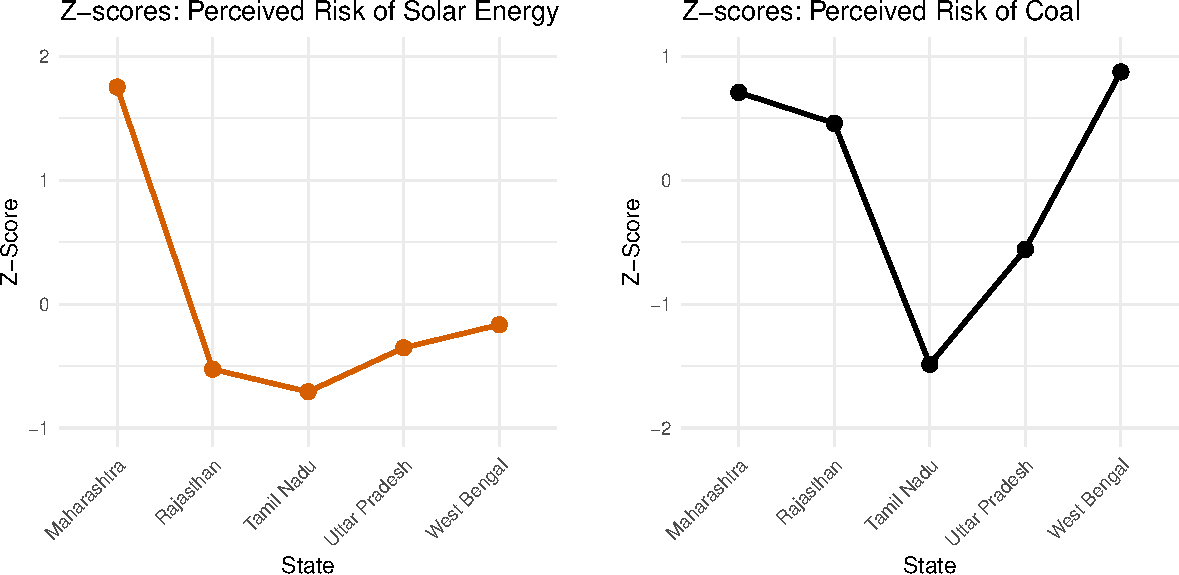
\includegraphics{nuclear-in-comparison_files/figure-latex/unnamed-chunk-34-2.pdf}

\newpage

\hypertarget{mean-perceived-benefit-and-z-scores-by-state}{%
\subsection{Mean Perceived Benefit and Z-scores by
State}\label{mean-perceived-benefit-and-z-scores-by-state}}

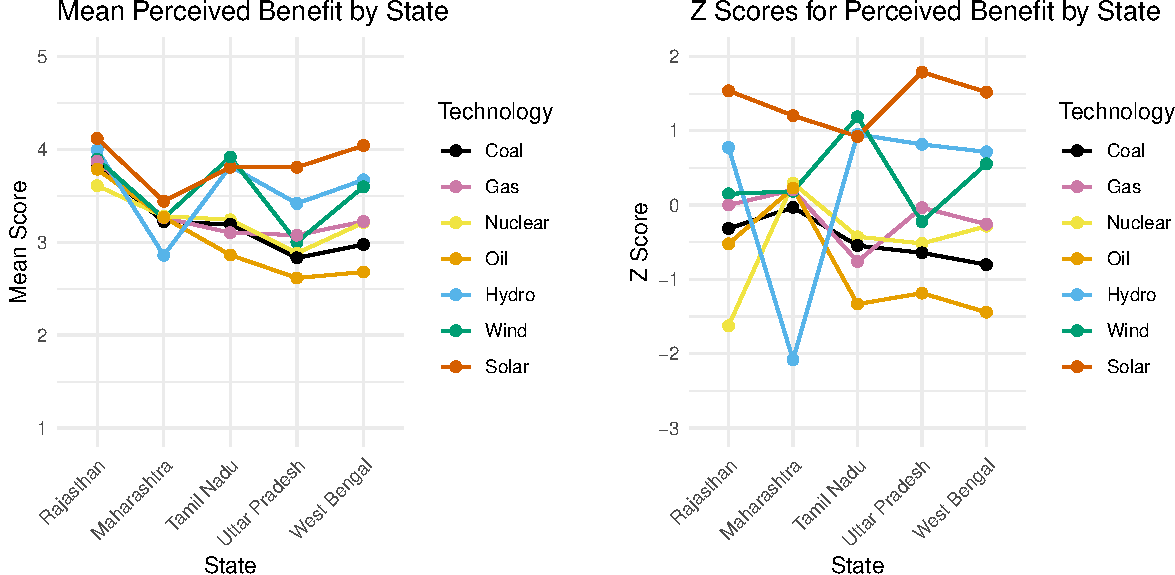
\includegraphics[width=1\linewidth,height=1\textheight]{nuclear-in-comparison_files/figure-latex/unnamed-chunk-37-1}

\newpage

\hypertarget{mean-perceived-benefit-and-z-scores-by-state---coal-solar-and-nuclear}{%
\subsection{Mean Perceived Benefit and Z-scores by State - coal solar
and
nuclear}\label{mean-perceived-benefit-and-z-scores-by-state---coal-solar-and-nuclear}}

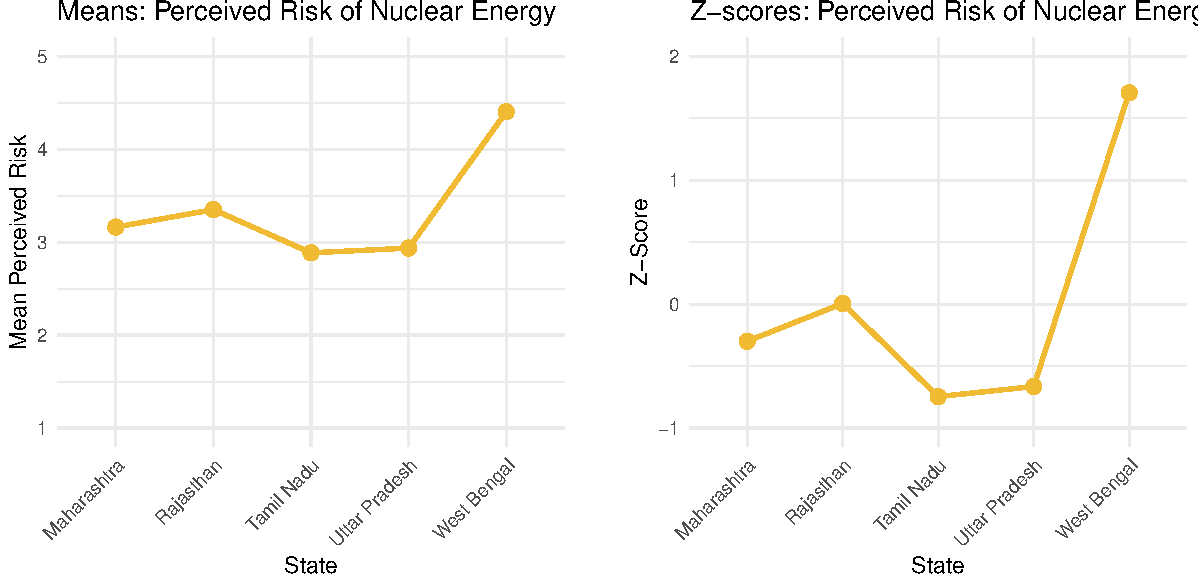
\includegraphics{nuclear-in-comparison_files/figure-latex/unnamed-chunk-38-1.pdf}

\newpage

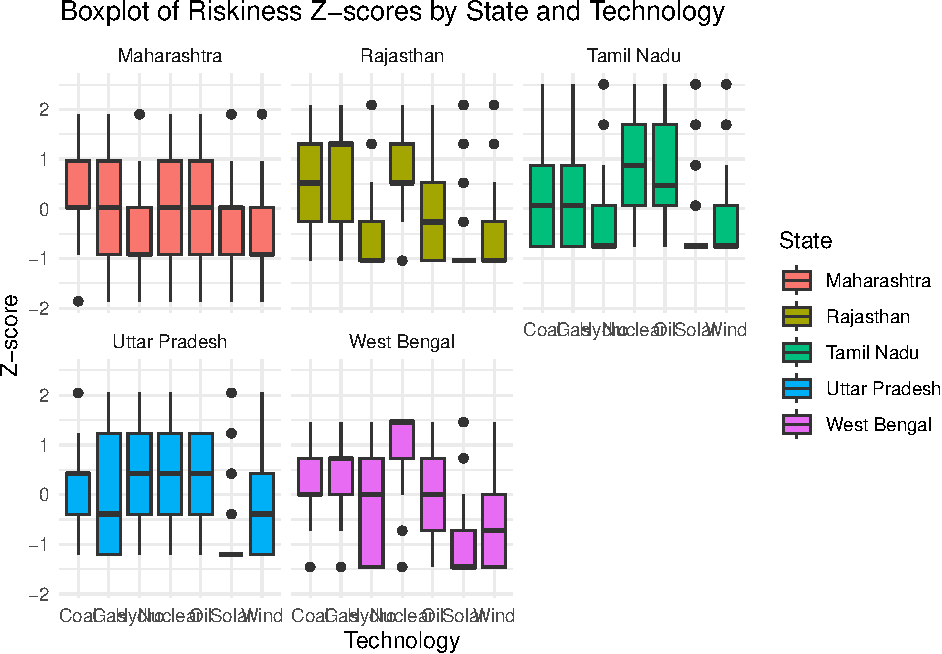
\includegraphics{nuclear-in-comparison_files/figure-latex/unnamed-chunk-40-1.pdf}
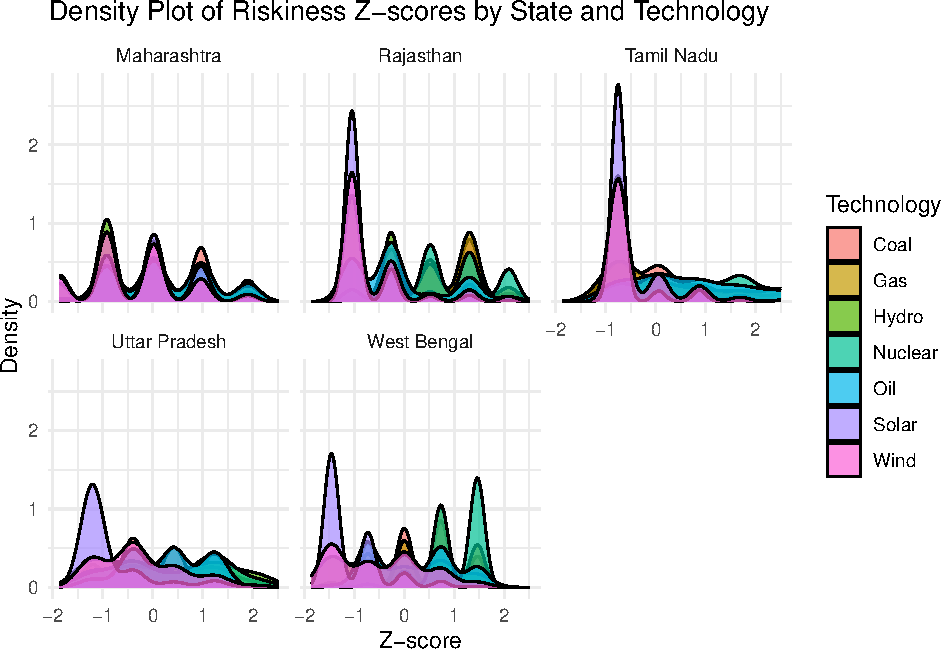
\includegraphics{nuclear-in-comparison_files/figure-latex/unnamed-chunk-40-2.pdf}
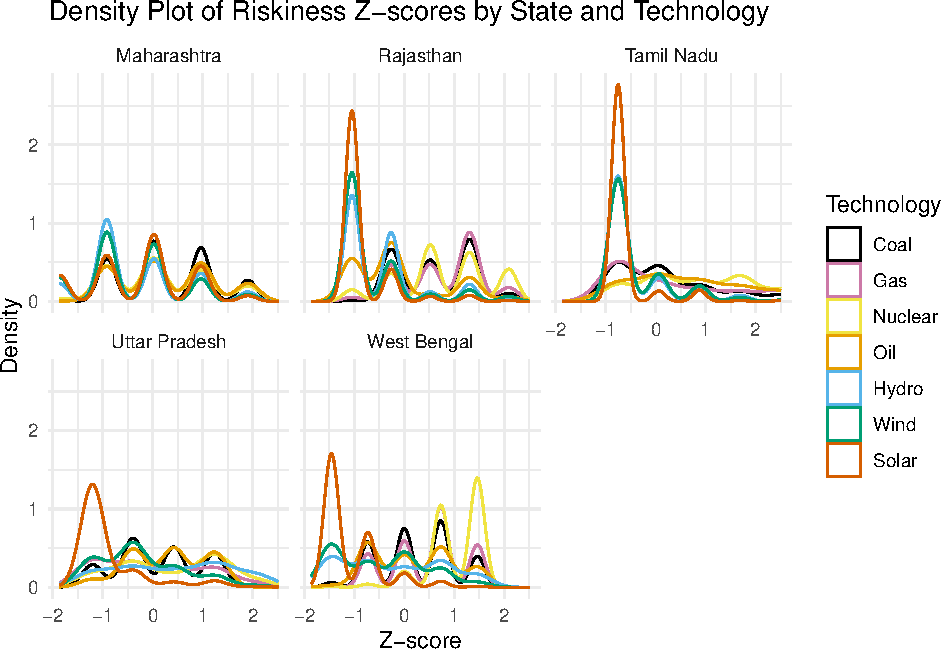
\includegraphics{nuclear-in-comparison_files/figure-latex/unnamed-chunk-40-3.pdf}
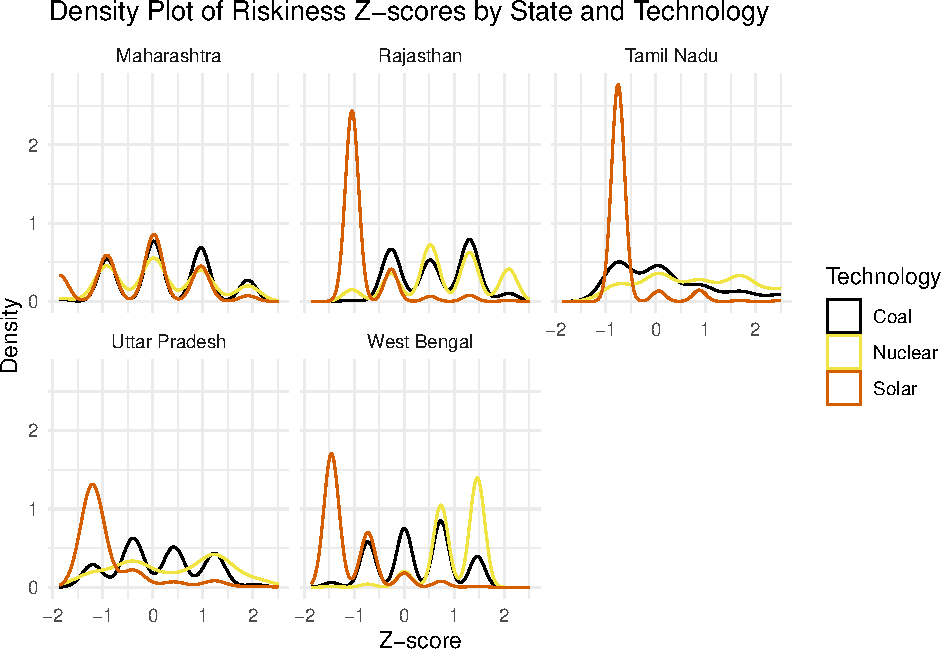
\includegraphics{nuclear-in-comparison_files/figure-latex/unnamed-chunk-40-4.pdf}

\begin{landscape}
\newpage

\hypertarget{linear-regression-perceived-risk-and-net-benefit--demographic-variables-including-state}{%
\subsection{Linear Regression : Perceived Risk and Net Benefit-
demographic variables including
State}\label{linear-regression-perceived-risk-and-net-benefit--demographic-variables-including-state}}

\begingroup\small\setlength{\tabcolsep}{1pt}

\renewcommand{\arraystretch}{0.7}

\% Table created by stargazer v.5.2.3 by Marek Hlavac, Social Policy
Institute. E-mail: marek.hlavac at gmail.com \% Date and time: Sun, Mar
24, 2024 - 13:06:02

\begin{table}[!htbp] \centering 
  \caption{Linear Models: Perceived Risk and Net Perceived Benefit(Nuclear, Solar and Coal)} 
  \label{} 
\begin{tabular}{@{\extracolsep{5pt}}lcccccc} 
\\[-1.8ex]\hline 
\hline \\[-1.8ex] 
 & \multicolumn{6}{c}{\textit{Dependent variable:}} \\ 
\cline{2-7} 
\\[-1.8ex] & RiskNuclear & RiskSolar & RiskCoal & NetBenNuclear & NetBenSolar & NetBenCoal \\ 
\\[-1.8ex] & (1) & (2) & (3) & (4) & (5) & (6)\\ 
\hline \\[-1.8ex] 
 Uppercaste & $-$0.135$^{**}$ & $-$0.006 & $-$0.056 & 0.026 & $-$0.146$^{*}$ & $-$0.021 \\ 
  & (0.061) & (0.051) & (0.058) & (0.089) & (0.084) & (0.075) \\ 
  & & & & & & \\ 
 Male & 0.045 & $-$0.047 & 0.015 & 0.008 & 0.058 & $-$0.016 \\ 
  & (0.062) & (0.053) & (0.059) & (0.092) & (0.087) & (0.078) \\ 
  & & & & & & \\ 
 Hindu & $-$0.047 & $-$0.057 & 0.099 & 0.362$^{***}$ & 0.290$^{***}$ & $-$0.008 \\ 
  & (0.070) & (0.059) & (0.066) & (0.100) & (0.095) & (0.085) \\ 
  & & & & & & \\ 
 UrbanUrban & 0.052 & $-$0.076 & 0.055 & 0.172$^{*}$ & 0.143 & 0.014 \\ 
  & (0.067) & (0.056) & (0.063) & (0.099) & (0.093) & (0.084) \\ 
  & & & & & & \\ 
 age & $-$0.015 & 0.045$^{**}$ & 0.053$^{**}$ & $-$0.008 & 0.045 & $-$0.035 \\ 
  & (0.027) & (0.023) & (0.025) & (0.043) & (0.040) & (0.036) \\ 
  & & & & & & \\ 
 StateRajasthan & 0.222$^{**}$ & $-$1.285$^{***}$ & 0.234$^{***}$ & $-$0.014 & 1.957$^{***}$ & 0.077 \\ 
  & (0.094) & (0.080) & (0.090) & (0.135) & (0.128) & (0.115) \\ 
  & & & & & & \\ 
 StateTamil Nadu & $-$0.242$^{**}$ & $-$1.547$^{***}$ & $-$1.103$^{***}$ & $-$0.625$^{***}$ & 2.027$^{***}$ & 0.795$^{***}$ \\ 
  & (0.099) & (0.084) & (0.094) & (0.191) & (0.181) & (0.162) \\ 
  & & & & & & \\ 
 StateUttar Pradesh & $-$0.178 & $-$1.344$^{***}$ & $-$0.638$^{***}$ & $-$0.250 & 1.612$^{***}$ & 0.296$^{**}$ \\ 
  & (0.120) & (0.102) & (0.114) & (0.177) & (0.168) & (0.151) \\ 
  & & & & & & \\ 
 StateWest Bengal & 1.276$^{***}$ & $-$1.330$^{***}$ & 0.071 & $-$1.522$^{***}$ & 1.853$^{***}$ & $-$0.222$^{**}$ \\ 
  & (0.083) & (0.071) & (0.079) & (0.125) & (0.118) & (0.106) \\ 
  & & & & & & \\ 
 Constant & 3.208$^{***}$ & 2.752$^{***}$ & 3.053$^{***}$ & $-$0.240 & 0.323$^{**}$ & 0.022 \\ 
  & (0.100) & (0.084) & (0.095) & (0.147) & (0.139) & (0.124) \\ 
  & & & & & & \\ 
\hline \\[-1.8ex] 
Observations & 1,444 & 1,444 & 1,444 & 1,183 & 1,183 & 1,183 \\ 
R$^{2}$ & 0.204 & 0.353 & 0.141 & 0.171 & 0.338 & 0.035 \\ 
Adjusted R$^{2}$ & 0.199 & 0.349 & 0.136 & 0.165 & 0.333 & 0.028 \\ 
Residual Std. Error & 1.057 (df = 1434) & 0.894 (df = 1434) & 1.004 (df = 1434) & 1.413 (df = 1173) & 1.334 (df = 1173) & 1.199 (df = 1173) \\ 
F Statistic & 40.720$^{***}$ (df = 9; 1434) & 86.983$^{***}$ (df = 9; 1434) & 26.208$^{***}$ (df = 9; 1434) & 26.873$^{***}$ (df = 9; 1173) & 66.499$^{***}$ (df = 9; 1173) & 4.789$^{***}$ (df = 9; 1173) \\ 
\hline 
\hline \\[-1.8ex] 
\textit{Note:}  & \multicolumn{6}{r}{$^{*}$p$<$0.1; $^{**}$p$<$0.05; $^{***}$p$<$0.01} \\ 
\end{tabular} 
\end{table} 
\endgroup

Linear Models: Perceived Risk and Net Perceived Benefit (Nuclear, Solar
and Coal)

Dependent variable:

RiskNuclear

RiskSolar

RiskCoal

NetBenNuclear

NetBenSolar

NetBenCoal

(1)

(2)

(3)

(4)

(5)

(6)

Uppercaste

-0.135**

-0.006

-0.056

0.026

-0.146*

-0.021

(0.061)

(0.051)

(0.058)

(0.089)

(0.084)

(0.075)

Male

0.045

-0.047

0.015

0.008

0.058

-0.016

(0.062)

(0.053)

(0.059)

(0.092)

(0.087)

(0.078)

Hindu

-0.047

-0.057

0.099

0.362***

0.290***

-0.008

(0.070)

(0.059)

(0.066)

(0.100)

(0.095)

(0.085)

UrbanUrban

0.052

-0.076

0.055

0.172*

0.143

0.014

(0.067)

(0.056)

(0.063)

(0.099)

(0.093)

(0.084)

age

-0.015

0.045**

0.053**

-0.008

0.045

-0.035

(0.027)

(0.023)

(0.025)

(0.043)

(0.040)

(0.036)

StateRajasthan

0.222**

-1.285***

0.234***

-0.014

1.957***

0.077

(0.094)

(0.080)

(0.090)

(0.135)

(0.128)

(0.115)

StateTamil Nadu

-0.242**

-1.547***

-1.103***

-0.625***

2.027***

0.795***

(0.099)

(0.084)

(0.094)

(0.191)

(0.181)

(0.162)

StateUttar Pradesh

-0.178

-1.344***

-0.638***

-0.250

1.612***

0.296**

(0.120)

(0.102)

(0.114)

(0.177)

(0.168)

(0.151)

StateWest Bengal

1.276***

-1.330***

0.071

-1.522***

1.853***

-0.222**

(0.083)

(0.071)

(0.079)

(0.125)

(0.118)

(0.106)

Constant

3.208***

2.752***

3.053***

-0.240

0.323**

0.022

(0.100)

(0.084)

(0.095)

(0.147)

(0.139)

(0.124)

Observations

1,444

1,444

1,444

1,183

1,183

1,183

R2

0.204

0.353

0.141

0.171

0.338

0.035

Adjusted R2

0.199

0.349

0.136

0.165

0.333

0.028

Residual Std. Error

1.057 (df = 1434)

0.894 (df = 1434)

1.004 (df = 1434)

1.413 (df = 1173)

1.334 (df = 1173)

1.199 (df = 1173)

F Statistic

40.720*** (df = 9; 1434)

86.983*** (df = 9; 1434)

26.208*** (df = 9; 1434)

26.873*** (df = 9; 1173)

66.499*** (df = 9; 1173)

4.789*** (df = 9; 1173)

Note:

\emph{p\textless0.1; \textbf{p\textless0.05; }}p\textless0.01

\end{landscape}

\begin{verbatim}
## 
## Regression Models Summary
## ========================================================================================================================================================================
##                                                                                     Dependent variable:                                                                 
##                     ----------------------------------------------------------------------------------------------------------------------------------------------------
##                           RiskNuclear               RiskSolar                 RiskCoal              NetBenNuclear             NetBenSolar              NetBenCoal       
##                               (1)                      (2)                      (3)                      (4)                      (5)                      (6)          
## ------------------------------------------------------------------------------------------------------------------------------------------------------------------------
## Uppercaste                  -0.135**                  -0.006                   -0.056                   0.026                   -0.146*                  -0.021         
##                             (0.061)                  (0.051)                  (0.058)                  (0.089)                  (0.084)                  (0.075)        
##                                                                                                                                                                         
## Male                         0.045                    -0.047                   0.015                    0.008                    0.058                   -0.016         
##                             (0.062)                  (0.053)                  (0.059)                  (0.092)                  (0.087)                  (0.078)        
##                                                                                                                                                                         
## Hindu                        -0.047                   -0.057                   0.099                   0.362***                 0.290***                 -0.008         
##                             (0.070)                  (0.059)                  (0.066)                  (0.100)                  (0.095)                  (0.085)        
##                                                                                                                                                                         
## UrbanUrban                   0.052                    -0.076                   0.055                    0.172*                   0.143                    0.014         
##                             (0.067)                  (0.056)                  (0.063)                  (0.099)                  (0.093)                  (0.084)        
##                                                                                                                                                                         
## age                          -0.015                  0.045**                  0.053**                   -0.008                   0.045                   -0.035         
##                             (0.027)                  (0.023)                  (0.025)                  (0.043)                  (0.040)                  (0.036)        
##                                                                                                                                                                         
## StateRajasthan              0.222**                 -1.285***                 0.234***                  -0.014                  1.957***                  0.077         
##                             (0.094)                  (0.080)                  (0.090)                  (0.135)                  (0.128)                  (0.115)        
##                                                                                                                                                                         
## StateTamil Nadu             -0.242**                -1.547***                -1.103***                -0.625***                 2.027***                0.795***        
##                             (0.099)                  (0.084)                  (0.094)                  (0.191)                  (0.181)                  (0.162)        
##                                                                                                                                                                         
## StateUttar Pradesh           -0.178                 -1.344***                -0.638***                  -0.250                  1.612***                 0.296**        
##                             (0.120)                  (0.102)                  (0.114)                  (0.177)                  (0.168)                  (0.151)        
##                                                                                                                                                                         
## StateWest Bengal            1.276***                -1.330***                  0.071                  -1.522***                 1.853***                -0.222**        
##                             (0.083)                  (0.071)                  (0.079)                  (0.125)                  (0.118)                  (0.106)        
##                                                                                                                                                                         
## Constant                    3.208***                 2.752***                 3.053***                  -0.240                  0.323**                   0.022         
##                             (0.100)                  (0.084)                  (0.095)                  (0.147)                  (0.139)                  (0.124)        
##                                                                                                                                                                         
## ------------------------------------------------------------------------------------------------------------------------------------------------------------------------
## Observations                 1,444                    1,444                    1,444                    1,183                    1,183                    1,183         
## R2                           0.204                    0.353                    0.141                    0.171                    0.338                    0.035         
## Adjusted R2                  0.199                    0.349                    0.136                    0.165                    0.333                    0.028         
## Residual Std. Error    1.057 (df = 1434)        0.894 (df = 1434)        1.004 (df = 1434)        1.413 (df = 1173)        1.334 (df = 1173)        1.199 (df = 1173)   
## F Statistic         40.720*** (df = 9; 1434) 86.983*** (df = 9; 1434) 26.208*** (df = 9; 1434) 26.873*** (df = 9; 1173) 66.499*** (df = 9; 1173) 4.789*** (df = 9; 1173)
## ========================================================================================================================================================================
## Note:                                                                                                                                        *p<0.1; **p<0.05; ***p<0.01
\end{verbatim}

\newpage

\hypertarget{claim-3-cultural-political-and-economic-values}{%
\section{Claim 3: Cultural, Political and Economic
Values}\label{claim-3-cultural-political-and-economic-values}}

\hypertarget{cfa-on-eco-pol-scale-for-solar-energy}{%
\subsection{CFA on eco-pol scale for Solar
Energy}\label{cfa-on-eco-pol-scale-for-solar-energy}}

\begin{landscape}\begin{table}[!h]

\caption{\label{tab:unnamed-chunk-49}Confirmatory Factor Analysis(CFA) on newly developed eco-pol scale}
\centering
\resizebox{\linewidth}{!}{
\begin{tabular}[t]{l>{\raggedright\arraybackslash}p{4cm}rrrrrrrr}
\toprule
Scale & Items & Loadings & Standard Error & zvalue & pvalue & ci.lower & ci.upper & std.lv & std.all\\
\midrule
\cellcolor{gray!6}{People Centered Development} & \cellcolor{gray!6}{Solar energy poses a great risk to the health of people living around it.} & \cellcolor{gray!6}{0.965} & \cellcolor{gray!6}{0.050} & \cellcolor{gray!6}{19.455} & \cellcolor{gray!6}{0e+00} & \cellcolor{gray!6}{0.8678100} & \cellcolor{gray!6}{1.0622499} & \cellcolor{gray!6}{0.9650299} & \cellcolor{gray!6}{0.7747043}\\
People Centered Development & Solar energy spoils the natural beauty of the landscape. & 0.820 & 0.052 & 15.714 & 0e+00 & 0.7177752 & 0.9223481 & 0.8200617 & 0.6560430\\
\cellcolor{gray!6}{People Centered Development} & \cellcolor{gray!6}{Solar energy is leading to displacement of people from their land.} & \cellcolor{gray!6}{0.692} & \cellcolor{gray!6}{0.050} & \cellcolor{gray!6}{13.800} & \cellcolor{gray!6}{0e+00} & \cellcolor{gray!6}{0.5939852} & \cellcolor{gray!6}{0.7906393} & \cellcolor{gray!6}{0.6923123} & \cellcolor{gray!6}{0.5906886}\\
People Centered Development & Solar energy increases pollution of air/water/land. & 1.096 & 0.050 & 21.706 & 0e+00 & 0.9970923 & 1.1950355 & 1.0960639 & 0.8411179\\
\cellcolor{gray!6}{People Centered Development} & \cellcolor{gray!6}{Large corporations are destroying the local industries in India and benefiting only a handful of people.} & \cellcolor{gray!6}{-0.287} & \cellcolor{gray!6}{0.058} & \cellcolor{gray!6}{-4.972} & \cellcolor{gray!6}{7e-07} & \cellcolor{gray!6}{-0.4007040} & \cellcolor{gray!6}{-0.1741052} & \cellcolor{gray!6}{-0.2874046} & \cellcolor{gray!6}{-0.2317296}\\
\addlinespace
People Centered Development & Regardless of ownership, the government should pass strong regulations and implement them. & -0.296 & 0.052 & -5.733 & 0e+00 & -0.3974941 & -0.1949541 & -0.2962241 & -0.2659785\\
\cellcolor{gray!6}{Nationalist Development} & \cellcolor{gray!6}{MECHANISATION} & \cellcolor{gray!6}{-0.445} & \cellcolor{gray!6}{0.052} & \cellcolor{gray!6}{-8.501} & \cellcolor{gray!6}{0e+00} & \cellcolor{gray!6}{-0.5481301} & \cellcolor{gray!6}{-0.3427323} & \cellcolor{gray!6}{-0.4454312} & \cellcolor{gray!6}{-0.3859243}\\
Nationalist Development & Solar energy pushes forward the country's development. & 1.042 & 0.046 & 22.549 & 0e+00 & 0.9518805 & 1.1331082 & 1.0424943 & 0.8341064\\
\cellcolor{gray!6}{Nationalist Development} & \cellcolor{gray!6}{I would be proud if my community used solar energy} & \cellcolor{gray!6}{1.042} & \cellcolor{gray!6}{0.047} & \cellcolor{gray!6}{21.934} & \cellcolor{gray!6}{0e+00} & \cellcolor{gray!6}{0.9485906} & \cellcolor{gray!6}{1.1347564} & \cellcolor{gray!6}{1.0416735} & \cellcolor{gray!6}{0.8187225}\\
Nationalist Development & Solar energy is a mark of pride for our nation. & 0.959 & 0.047 & 20.244 & 0e+00 & 0.8658229 & 1.0514501 & 0.9586365 & 0.7748161\\
\addlinespace
\cellcolor{gray!6}{Nationalist Development} & \cellcolor{gray!6}{Solar energy brings economic prosperity to the surrounding regions.} & \cellcolor{gray!6}{0.980} & \cellcolor{gray!6}{0.047} & \cellcolor{gray!6}{20.803} & \cellcolor{gray!6}{0e+00} & \cellcolor{gray!6}{0.8876975} & \cellcolor{gray!6}{1.0723692} & \cellcolor{gray!6}{0.9800333} & \cellcolor{gray!6}{0.7896156}\\
NA & Solar energy will bring jobs to the local community. & 0.641 & 0.051 & 12.542 & 0e+00 & 0.5406190 & 0.7408777 & 0.6407483 & 0.5339818\\
\cellcolor{gray!6}{NA} & \cellcolor{gray!6}{Solar energy poses a great risk to the health of people living around it.} & \cellcolor{gray!6}{0.620} & \cellcolor{gray!6}{0.054} & \cellcolor{gray!6}{11.424} & \cellcolor{gray!6}{0e+00} & \cellcolor{gray!6}{0.5139817} & \cellcolor{gray!6}{0.7268665} & \cellcolor{gray!6}{0.6204241} & \cellcolor{gray!6}{0.3998333}\\
\bottomrule
\end{tabular}}
\end{table}
\end{landscape}

\newpage

\hypertarget{cfa-on-eco-pol-scale-for-coal}{%
\subsection{CFA on eco-pol scale for
Coal}\label{cfa-on-eco-pol-scale-for-coal}}

\begin{landscape}\begin{table}[!h]

\caption{\label{tab:unnamed-chunk-53}Confirmatory Factor Analysis(CFA) on newly developed eco-pol scale}
\centering
\resizebox{\linewidth}{!}{
\begin{tabular}[t]{l>{\raggedright\arraybackslash}p{4cm}rrrrrrrr}
\toprule
Scale & Items & Loadings & Standard Error & zvalue & pvalue & ci.lower & ci.upper & std.lv & std.all\\
\midrule
\cellcolor{gray!6}{People Centered Development} & \cellcolor{gray!6}{Coal powered plants poses a great risk to the health of people living around it.} & \cellcolor{gray!6}{0.713} & \cellcolor{gray!6}{0.051} & \cellcolor{gray!6}{14.083} & \cellcolor{gray!6}{0.0e+00} & \cellcolor{gray!6}{0.6140727} & \cellcolor{gray!6}{0.8126265} & \cellcolor{gray!6}{0.7133496} & \cellcolor{gray!6}{0.6482214}\\
People Centered Development & Coal powered plants spoils the natural beauty of the landscape. & 0.714 & 0.048 & 14.818 & 0.0e+00 & 0.6198092 & 0.8087672 & 0.7142882 & 0.6750268\\
\cellcolor{gray!6}{People Centered Development} & \cellcolor{gray!6}{Coal powered plants is leading to displacement of people from their land.} & \cellcolor{gray!6}{0.628} & \cellcolor{gray!6}{0.055} & \cellcolor{gray!6}{11.376} & \cellcolor{gray!6}{0.0e+00} & \cellcolor{gray!6}{0.5195755} & \cellcolor{gray!6}{0.7358706} & \cellcolor{gray!6}{0.6277231} & \cellcolor{gray!6}{0.5432527}\\
People Centered Development & Coal powered plants increases pollution of air/water/land. & 0.640 & 0.041 & 15.561 & 0.0e+00 & 0.5590262 & 0.7201432 & 0.6395847 & 0.7014985\\
\cellcolor{gray!6}{People Centered Development} & \cellcolor{gray!6}{Large corporations are destroying the local industries in India and benefiting only a handful of people.} & \cellcolor{gray!6}{0.634} & \cellcolor{gray!6}{0.057} & \cellcolor{gray!6}{11.174} & \cellcolor{gray!6}{0.0e+00} & \cellcolor{gray!6}{0.5225822} & \cellcolor{gray!6}{0.7449013} & \cellcolor{gray!6}{0.6337417} & \cellcolor{gray!6}{0.5349921}\\
\addlinespace
People Centered Development & Regardless of ownership, the government should pass strong regulations and implement them. & 0.509 & 0.054 & 9.351 & 0.0e+00 & 0.4027047 & 0.6162708 & 0.5094877 & 0.4577641\\
\cellcolor{gray!6}{Nationalist Development} & \cellcolor{gray!6}{MECHANISATION} & \cellcolor{gray!6}{0.656} & \cellcolor{gray!6}{0.056} & \cellcolor{gray!6}{11.682} & \cellcolor{gray!6}{0.0e+00} & \cellcolor{gray!6}{0.5460463} & \cellcolor{gray!6}{0.7662170} & \cellcolor{gray!6}{0.6561317} & \cellcolor{gray!6}{0.5556245}\\
Nationalist Development & Coal powered plants pushes forward the country's development. & 0.626 & 0.055 & 11.326 & 0.0e+00 & 0.5177592 & 0.7344596 & 0.6261094 & 0.6242574\\
\cellcolor{gray!6}{Nationalist Development} & \cellcolor{gray!6}{Coal powered plants brings economic prosperity to the surrounding regions.} & \cellcolor{gray!6}{0.547} & \cellcolor{gray!6}{0.054} & \cellcolor{gray!6}{10.086} & \cellcolor{gray!6}{0.0e+00} & \cellcolor{gray!6}{0.4408772} & \cellcolor{gray!6}{0.6535573} & \cellcolor{gray!6}{0.5472172} & \cellcolor{gray!6}{0.5535687}\\
NA & Coal powered plants will bring jobs to the local community. & 0.472 & 0.054 & 8.776 & 0.0e+00 & 0.3667103 & 0.5776005 & 0.4721554 & 0.4834144\\
\addlinespace
\cellcolor{gray!6}{NA} & \cellcolor{gray!6}{PRIDECOAL} & \cellcolor{gray!6}{0.338} & \cellcolor{gray!6}{0.062} & \cellcolor{gray!6}{5.485} & \cellcolor{gray!6}{0.0e+00} & \cellcolor{gray!6}{0.2173242} & \cellcolor{gray!6}{0.4590249} & \cellcolor{gray!6}{0.3381745} & \cellcolor{gray!6}{0.3081207}\\
NA & NPRIDECOAL & 0.284 & 0.061 & 4.667 & 3.1e-06 & 0.1645514 & 0.4027991 & 0.2836753 & 0.2634176\\
\cellcolor{gray!6}{NA} & \cellcolor{gray!6}{Coal powered plants poses a great risk to the health of people living around it.} & \cellcolor{gray!6}{0.702} & \cellcolor{gray!6}{0.056} & \cellcolor{gray!6}{12.572} & \cellcolor{gray!6}{0.0e+00} & \cellcolor{gray!6}{0.5927046} & \cellcolor{gray!6}{0.8116380} & \cellcolor{gray!6}{0.7021713} & \cellcolor{gray!6}{0.5798090}\\
NA & Coal powered plants spoils the natural beauty of the landscape. & 0.610 & 0.050 & 12.173 & 0.0e+00 & 0.5113671 & 0.7076348 & 0.6095009 & 0.5443389\\
\cellcolor{gray!6}{NA} & \cellcolor{gray!6}{Coal powered plants is leading to displacement of people from their land.} & \cellcolor{gray!6}{0.941} & \cellcolor{gray!6}{0.069} & \cellcolor{gray!6}{13.656} & \cellcolor{gray!6}{0.0e+00} & \cellcolor{gray!6}{0.8060444} & \cellcolor{gray!6}{1.0761975} & \cellcolor{gray!6}{0.9411209} & \cellcolor{gray!6}{0.7048765}\\
\bottomrule
\end{tabular}}
\end{table}
\end{landscape}

\end{document}
